\hypertarget{backup_2dcs__driver_8c}{
\section{dcs\_\-driver.c File Reference}
\label{backup_2dcs__driver_8c}\index{dcs_driver.c@{dcs\_\-driver.c}}
}
{\tt \#include $<$linux/fs.h$>$}\par
{\tt \#include $<$linux/types.h$>$}\par
{\tt \#include $<$linux/sched.h$>$}\par
{\tt \#include $<$linux/errno.h$>$}\par
{\tt \#include $<$linux/slab.h$>$}\par
{\tt \#include $<$asm/io.h$>$}\par
{\tt \#include $<$asm/uaccess.h$>$}\par
{\tt \#include $<$linux/mm.h$>$}\par
{\tt \#include $<$linux/ioport.h$>$}\par
{\tt \#include $<$linux/spinlock.h$>$}\par
{\tt \#include $<$asm/system.h$>$}\par
{\tt \#include $<$linux/module.h$>$}\par
{\tt \#include \char`\"{}dcs\_\-driver.h\char`\"{}}\par
{\tt \#include \char`\"{}version.h\char`\"{}}\par
{\tt \#include \char`\"{}mr\-Kern\-Logging.c\char`\"{}}\par


Include dependency graph for backup/dcs\_\-driver.c:\begin{figure}[H]
\begin{center}
\leavevmode
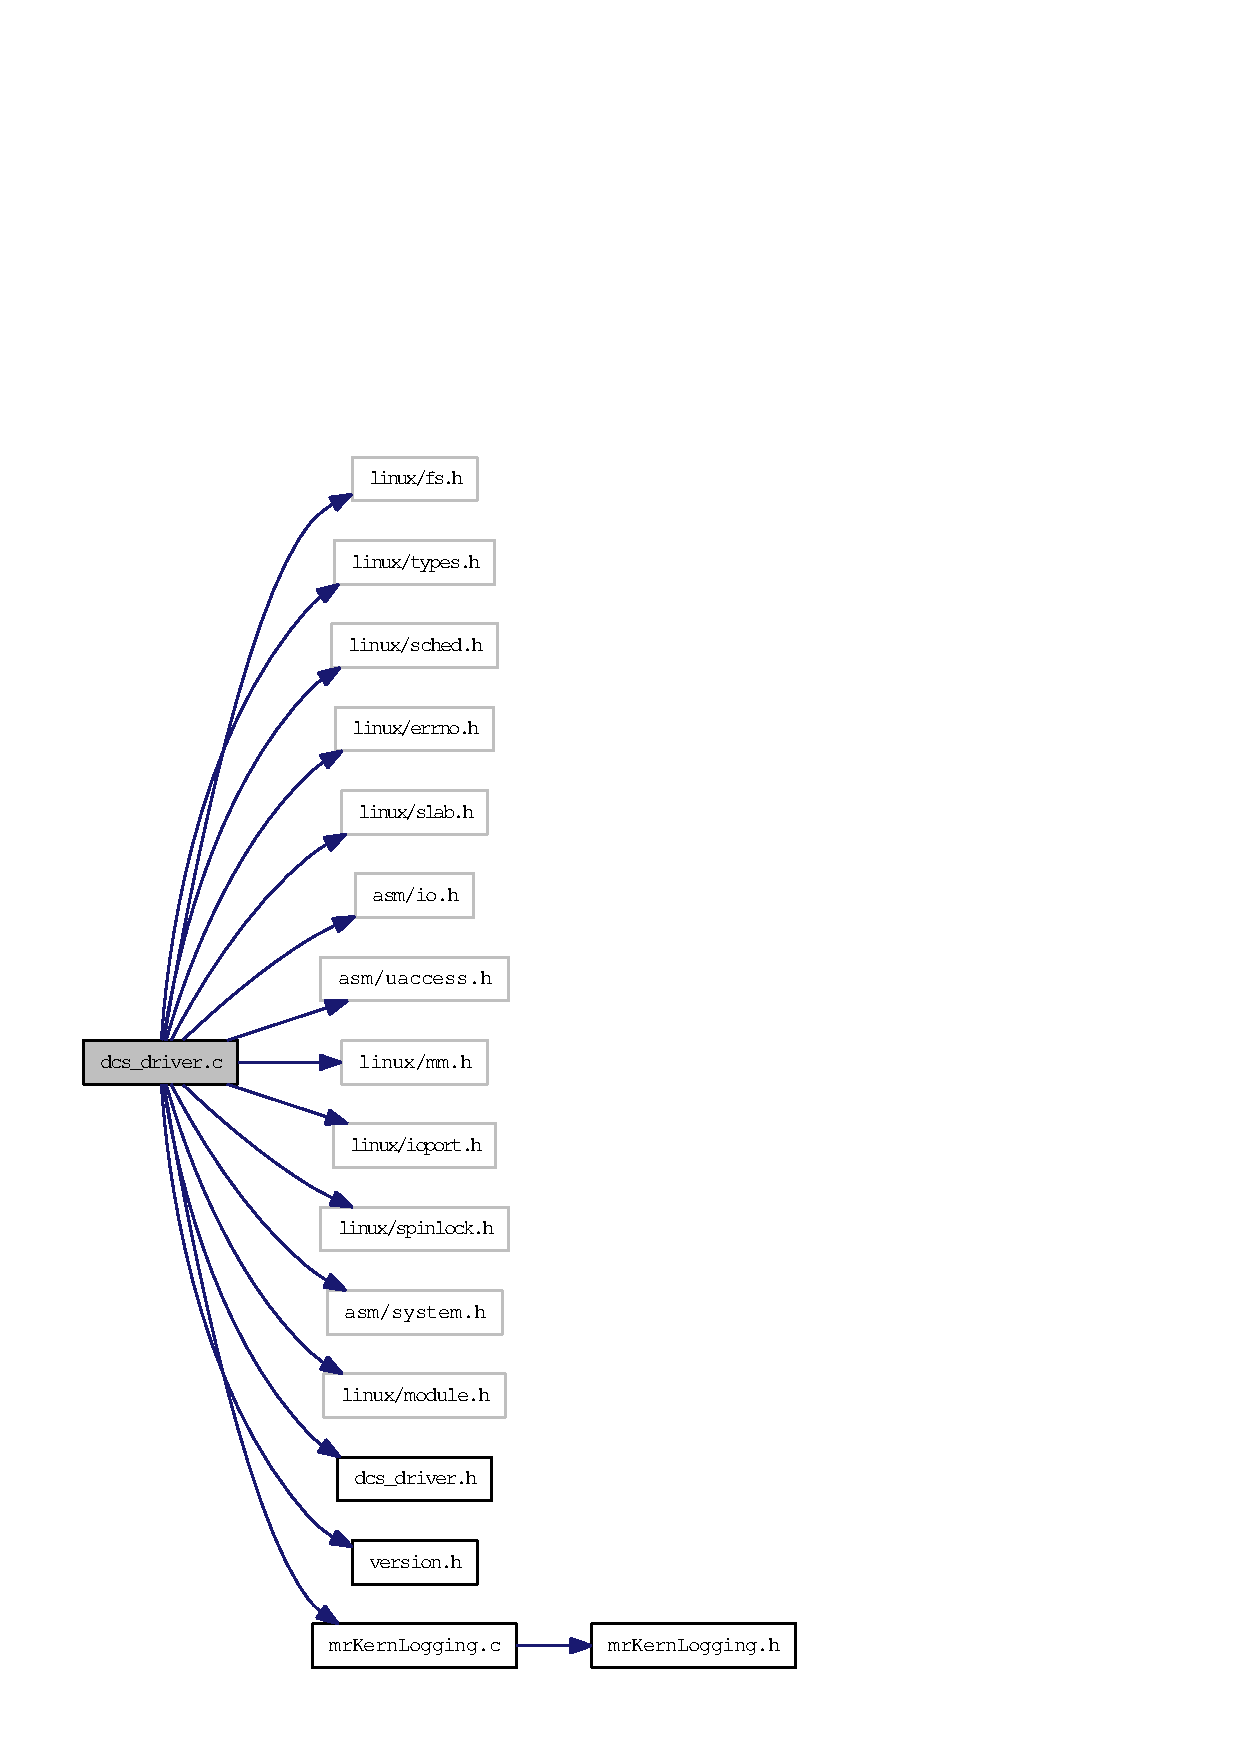
\includegraphics[width=193pt]{backup_2dcs__driver_8c__incl}
\end{center}
\end{figure}
\subsection*{Defines}
\begin{CompactItemize}
\item 
\#define \hyperlink{backup_2dcs__driver_8c_805e10412728f32d8585dd436b22cc99}{TEST\_\-PATTERN}~0x13071972
\end{CompactItemize}
\subsection*{Functions}
\begin{CompactItemize}
\item 
\hyperlink{backup_2dcs__driver_8c_3053a7067223a09a392be7f5871f9766}{MODULE\_\-PARM} (\hyperlink{dcs__driver_8c_45c631d40e14d14a309abbe2b87ccd1b}{dcsc\_\-major\-ID},\char`\"{}i\char`\"{})
\item 
\hyperlink{backup_2dcs__driver_8c_75f25d27ddf2830f44e578fb39146b97}{MODULE\_\-PARM} (\hyperlink{dcs__driver_8c_9a8b5688625d4564010909cb4e23192f}{dcsc\_\-msgbuf\_\-in\_\-size},\char`\"{}i\char`\"{})
\item 
\hyperlink{backup_2dcs__driver_8c_d2a9008a63b5fc661f4aa83a8a0f8bcc}{MODULE\_\-PARM} (\hyperlink{dcs__driver_8c_57243357aaca143dc0a0e93dcd16eb89}{dcsc\_\-msgbuf\_\-out\_\-size},\char`\"{}i\char`\"{})
\item 
\hyperlink{backup_2dcs__driver_8c_19e37b390f71b35e88960d78c6d836c4}{MODULE\_\-PARM} (\hyperlink{dcs__driver_8c_898ab396bb466832c0c38ecc37f16632}{dcsc\_\-regfile\_\-size},\char`\"{}i\char`\"{})
\item 
\hyperlink{backup_2dcs__driver_8c_73936caf0f944aa65a75a16e077c835a}{MODULE\_\-PARM} (\hyperlink{dcs__driver_8c_03af36d4209f6364a9f7a5f1087f19f9}{msgbuf\_\-in\_\-physaddr},\char`\"{}i\char`\"{})
\item 
\hyperlink{backup_2dcs__driver_8c_b8f38a668f504ecdbf2041c14fc8f50f}{MODULE\_\-PARM} (\hyperlink{dcs__driver_8c_89c68fc835da1b91e1d93eecb77922b6}{msgbuf\_\-out\_\-physaddr},\char`\"{}i\char`\"{})
\item 
\hyperlink{backup_2dcs__driver_8c_84a8ddb935ced6da7bdd97965f36cead}{MODULE\_\-PARM} (\hyperlink{dcs__driver_8c_607a6fb1f19bf1e11ec4fa99dc7efecd}{regfile\_\-physaddr},\char`\"{}i\char`\"{})
\item 
\hyperlink{backup_2dcs__driver_8c_53fff30413e173391c35bdc5481c1719}{MODULE\_\-AUTHOR} (\char`\"{}Matthias Richter\char`\"{})
\item 
\hyperlink{backup_2dcs__driver_8c_2eb38dffd9d03b7908c57b56ae9e9377}{MODULE\_\-DESCRIPTION} (\char`\"{}dcs-card register driver\char`\"{})
\item 
\hyperlink{backup_2dcs__driver_8c_d94b36675e7eb067ea3ce6ff9e244a44}{MODULE\_\-LICENSE} (\char`\"{}GPL\char`\"{})
\item 
static int \hyperlink{backup_2dcs__driver_8c_5fc9e61f41c571cca4373a64ca28d159}{memtest} (u32 begin, u32 size)
\item 
static int \hyperlink{backup_2dcs__driver_8c_24611c859ab5512627f0ebe5e71bb7df}{dcs\_\-comparevalue} (u32 begin, u32 size, u32 value)
\item 
static int \hyperlink{backup_2dcs__driver_8c_aec6947dd189feeedeb22af3fbc21d81}{dcs\_\-writevalue} (u32 begin, u32 size, u32 value)
\item 
static int \hyperlink{backup_2dcs__driver_8c_85874c4901b4b811c882944a3f77ff0e}{dcs\_\-read} (u32 begin, u32 size, u32 $\ast$buff)
\item 
static int \hyperlink{backup_2dcs__driver_8c_626a935595dad9fb4ce5cfdf4fd48f28}{dcs\_\-write} (u32 begin, u32 size, u32 $\ast$buff)
\item 
u32 \hyperlink{backup_2dcs__driver_8c_0f2edb55399fbd36008bbded20c5ecab}{find\-Buffer\-For\-Address} (loff\_\-t offset, int \hyperlink{dcs__driver_8c_269775bb092dfa3a11844c3d1883d988}{i\-Access\-Mode}, u32 $\ast$$\ast$pp\-Buffer, u32 $\ast$p\-Position, const char $\ast$$\ast$pp\-Buffer\-Name)
\item 
int \hyperlink{backup_2dcs__driver_8c_c619293d4edc146efb03fb6b03f8461f}{Init\-Driver\-Lock} ()
\item 
int \hyperlink{backup_2dcs__driver_8c_a754eaa169b47cb26cf5e997276ebd81}{lock\-Activate} ()
\item 
int \hyperlink{backup_2dcs__driver_8c_bfe7c9dd41295bc3fe20fc96aa3ac39d}{lock\-Reset} ()
\item 
int \hyperlink{backup_2dcs__driver_8c_4a2481d7c54d6ec0d99bc8716a8a021f}{check\-And\-Lock} (int i\-Seize\-Code, int pid)
\begin{CompactList}\small\item\em spin-lock protected check of the lock status variable. \item\end{CompactList}\item 
int \hyperlink{backup_2dcs__driver_8c_69f4b1ea76e4eeed7eb2fed3adc6e847}{lock\-Driver} (int i\-Seize\-Code, int i\-Time\-Out)
\begin{CompactList}\small\item\em Try to lock the driver, go to sleep if already locked. \item\end{CompactList}\item 
int \hyperlink{backup_2dcs__driver_8c_f65c837b7c30c1d6c4861e5dbb9a4e59}{seize\-Driver} (int i\-Seize\-Code)
\begin{CompactList}\small\item\em Lock the driver to a single application. \item\end{CompactList}\item 
int \hyperlink{backup_2dcs__driver_8c_0e119609dea51ec090e7852dd9d0abad}{unlock\-Driver} ()
\begin{CompactList}\small\item\em Unlock the driver and wake up all sleeping processes. \item\end{CompactList}\item 
int \hyperlink{backup_2dcs__driver_8c_6ccbabe02e6e0af40d2b653b2a158d40}{release\-Driver} (int i\-Seize\-Code)
\begin{CompactList}\small\item\em Release the driver which was locked to a single application. \item\end{CompactList}\item 
static loff\_\-t \hyperlink{backup_2dcs__driver_8c_1b18195d839987757d645e7761bdfbc1}{dcsc\_\-llseek} (struct file $\ast$filp, loff\_\-t off, int ref)
\item 
static int \hyperlink{backup_2dcs__driver_8c_8067a5efccbb89b363e4b12d4249bb07}{dcsc\_\-read} (struct file $\ast$filp, char $\ast$buf, size\_\-t count, loff\_\-t $\ast$f\_\-pos)
\item 
static int \hyperlink{backup_2dcs__driver_8c_0c28bf0d1a698b2c9c598715bd37a9cb}{dcsc\_\-write} (struct file $\ast$filp, const char $\ast$buf, size\_\-t count, loff\_\-t $\ast$f\_\-pos)
\item 
static int \hyperlink{backup_2dcs__driver_8c_1fc34702f88baf2a47a0434f6ea9e0cb}{dcsc\_\-open} (struct inode $\ast$inode, struct file $\ast$filp)
\item 
static int \hyperlink{backup_2dcs__driver_8c_5350bab3f3d6d1f1e2c84ecafa150d68}{dcsc\_\-close} (struct inode $\ast$inode, struct file $\ast$filp)
\item 
static int \hyperlink{backup_2dcs__driver_8c_c3b4c74273847bef0006306f638cc133}{dcsc\_\-mmap} (struct file $\ast$filp, struct vm\_\-area\_\-struct $\ast$vma)
\item 
static int \hyperlink{backup_2dcs__driver_8c_30d7523911ed6cebd68b1d5c34da9d64}{dcsc\_\-ioctl} (struct inode $\ast$inode, struct file $\ast$filp, unsigned int cmd, unsigned long arg)
\item 
void \hyperlink{backup_2dcs__driver_8c_06a93d1b1348b354639233cdab90e9fe}{cleanup\-Real\-Buffers} ()
\item 
int \hyperlink{backup_2dcs__driver_8c_b3161c882ef5359bf75cf6705c545cd4}{init\-Real\-Buffers} ()
\item 
int \hyperlink{backup_2dcs__driver_8c_e52690ce6969b799366b2c5feba67b8c}{init\_\-module} (void)
\item 
void \hyperlink{backup_2dcs__driver_8c_bb8e1606224e802418862b898888063a}{cleanup\_\-module} (void)
\end{CompactItemize}
\subsection*{Variables}
\begin{CompactItemize}
\item 
int \hyperlink{backup_2dcs__driver_8c_45c631d40e14d14a309abbe2b87ccd1b}{dcsc\_\-major\-ID} = 150
\item 
static int \hyperlink{backup_2dcs__driver_8c_9a8b5688625d4564010909cb4e23192f}{dcsc\_\-msgbuf\_\-in\_\-size} = 0x400
\item 
static int \hyperlink{backup_2dcs__driver_8c_57243357aaca143dc0a0e93dcd16eb89}{dcsc\_\-msgbuf\_\-out\_\-size} = 0x400
\item 
static int \hyperlink{backup_2dcs__driver_8c_898ab396bb466832c0c38ecc37f16632}{dcsc\_\-regfile\_\-size} = 0x10
\item 
static u32 $\ast$ \hyperlink{backup_2dcs__driver_8c_03af36d4209f6364a9f7a5f1087f19f9}{msgbuf\_\-in\_\-physaddr} = ((u32 $\ast$) 0x80000400)
\item 
static u32 $\ast$ \hyperlink{backup_2dcs__driver_8c_89c68fc835da1b91e1d93eecb77922b6}{msgbuf\_\-out\_\-physaddr} = ((u32 $\ast$) 0x80000800)
\item 
static u32 $\ast$ \hyperlink{backup_2dcs__driver_8c_607a6fb1f19bf1e11ec4fa99dc7efecd}{regfile\_\-physaddr} = ((u32 $\ast$) 0x80000060)
\item 
static u32 $\ast$ \hyperlink{backup_2dcs__driver_8c_a6f29aaef9f61f455e1eeb2890ca8300}{msgbuf\_\-in\_\-virtbase} = NULL
\item 
static u32 $\ast$ \hyperlink{backup_2dcs__driver_8c_6bd1f1592c9416c2bb4de131829a232d}{msgbuf\_\-out\_\-virtbase} = NULL
\item 
static u32 $\ast$ \hyperlink{backup_2dcs__driver_8c_dd264756338f180733724b4ea909d1cf}{regfile\_\-virtbase} = NULL
\item 
static int \hyperlink{backup_2dcs__driver_8c_269775bb092dfa3a11844c3d1883d988}{i\-Access\-Mode} = ACCESS\_\-ALL
\item 
wait\_\-queue\_\-head\_\-t \hyperlink{backup_2dcs__driver_8c_c5ac2769997c4ac1e8307c4521c4b20e}{g\_\-wait\-Queue}
\item 
int \hyperlink{backup_2dcs__driver_8c_983d0af3572a91f1c34b942ff8954544}{g\_\-i\-Lock\-Reset} = 0
\item 
int \hyperlink{backup_2dcs__driver_8c_18b5596c6309017456c046d61b05e3b1}{g\_\-i\-Lock} = 0
\item 
int \hyperlink{backup_2dcs__driver_8c_750fd6e08c92777b860f11e575a4e804}{g\_\-i\-Lock\-Pid} = 0
\item 
int \hyperlink{backup_2dcs__driver_8c_2d3bbc70ca9389e34e840e3c3fade06d}{g\_\-i\-Seize\-Code} = 0
\item 
spinlock\_\-t \hyperlink{backup_2dcs__driver_8c_2f3f72c4a42056343b2c0ac401326cb4}{g\_\-spinlock}
\item 
int \hyperlink{backup_2dcs__driver_8c_c23aa679017a305c1a149016fea0c003}{g\_\-i\-Lock\-Initialized} = 0
\item 
file\_\-operations \hyperlink{backup_2dcs__driver_8c_010266ee96b0e2fd685de9f760d64dd8}{dcsc\_\-fops}
\end{CompactItemize}


\subsection{Define Documentation}
\hypertarget{backup_2dcs__driver_8c_805e10412728f32d8585dd436b22cc99}{
\index{backup/dcs_driver.c@{backup/dcs\_\-driver.c}!TEST_PATTERN@{TEST\_\-PATTERN}}
\index{TEST_PATTERN@{TEST\_\-PATTERN}!backup/dcs_driver.c@{backup/dcs\_\-driver.c}}
\subsubsection[TEST\_\-PATTERN]{\setlength{\rightskip}{0pt plus 5cm}\#define TEST\_\-PATTERN~0x13071972}}
\label{backup_2dcs__driver_8c_805e10412728f32d8585dd436b22cc99}




Definition at line 504 of file backup/dcs\_\-driver.c.

Referenced by init\-Real\-Buffers().

\subsection{Function Documentation}
\hypertarget{backup_2dcs__driver_8c_4a2481d7c54d6ec0d99bc8716a8a021f}{
\index{backup/dcs_driver.c@{backup/dcs\_\-driver.c}!checkAndLock@{checkAndLock}}
\index{checkAndLock@{checkAndLock}!backup/dcs_driver.c@{backup/dcs\_\-driver.c}}
\subsubsection[checkAndLock]{\setlength{\rightskip}{0pt plus 5cm}int check\-And\-Lock (int {\em i\-Seize\-Code}, int {\em pid})}}
\label{backup_2dcs__driver_8c_4a2481d7c54d6ec0d99bc8716a8a021f}


spin-lock protected check of the lock status variable. 

If the lock is free it will be set. If the lock is owned by the current process the lock is incremented. The driver can be {\em master\/} locked by an application which causes the lock to return {\em permission denied\/} for requests by other applications. \begin{Desc}
\item[Parameters:]
\begin{description}
\item[{\em i\-Seize\-Code}]master lock code given by the application \item[{\em i\-Time\-Out}]time out (currently not used) \end{description}
\end{Desc}
\begin{Desc}
\item[Returns:]1 if free and now set, 0 if already blocked\par
 -ETIMEDOUT if time out\par
 -EPERM driver in master lock \end{Desc}


Definition at line 334 of file backup/dcs\_\-driver.c.

References g\_\-i\-Lock, g\_\-i\-Lock\-Initialized, g\_\-i\-Lock\-Pid, g\_\-i\-Seize\-Code, g\_\-spinlock, LOG\_\-DBG, LOG\_\-DRIVER\_\-LCK, MR\_\-KERN\_\-DEBUG, and mrlogmessage().

Referenced by lock\-Driver().

Here is the call graph for this function:\begin{figure}[H]
\begin{center}
\leavevmode
\includegraphics[width=127pt]{backup_2dcs__driver_8c_4a2481d7c54d6ec0d99bc8716a8a021f_cgraph}
\end{center}
\end{figure}
\hypertarget{backup_2dcs__driver_8c_bb8e1606224e802418862b898888063a}{
\index{backup/dcs_driver.c@{backup/dcs\_\-driver.c}!cleanup_module@{cleanup\_\-module}}
\index{cleanup_module@{cleanup\_\-module}!backup/dcs_driver.c@{backup/dcs\_\-driver.c}}
\subsubsection[cleanup\_\-module]{\setlength{\rightskip}{0pt plus 5cm}void cleanup\_\-module (void)}}
\label{backup_2dcs__driver_8c_bb8e1606224e802418862b898888063a}




Definition at line 659 of file backup/dcs\_\-driver.c.

References cleanup\-Real\-Buffers(), cleanup\-Simulated\-Buffers(), dcsc\_\-major\-ID, LOG\_\-INFO, and mrlogmessage().

Here is the call graph for this function:\begin{figure}[H]
\begin{center}
\leavevmode
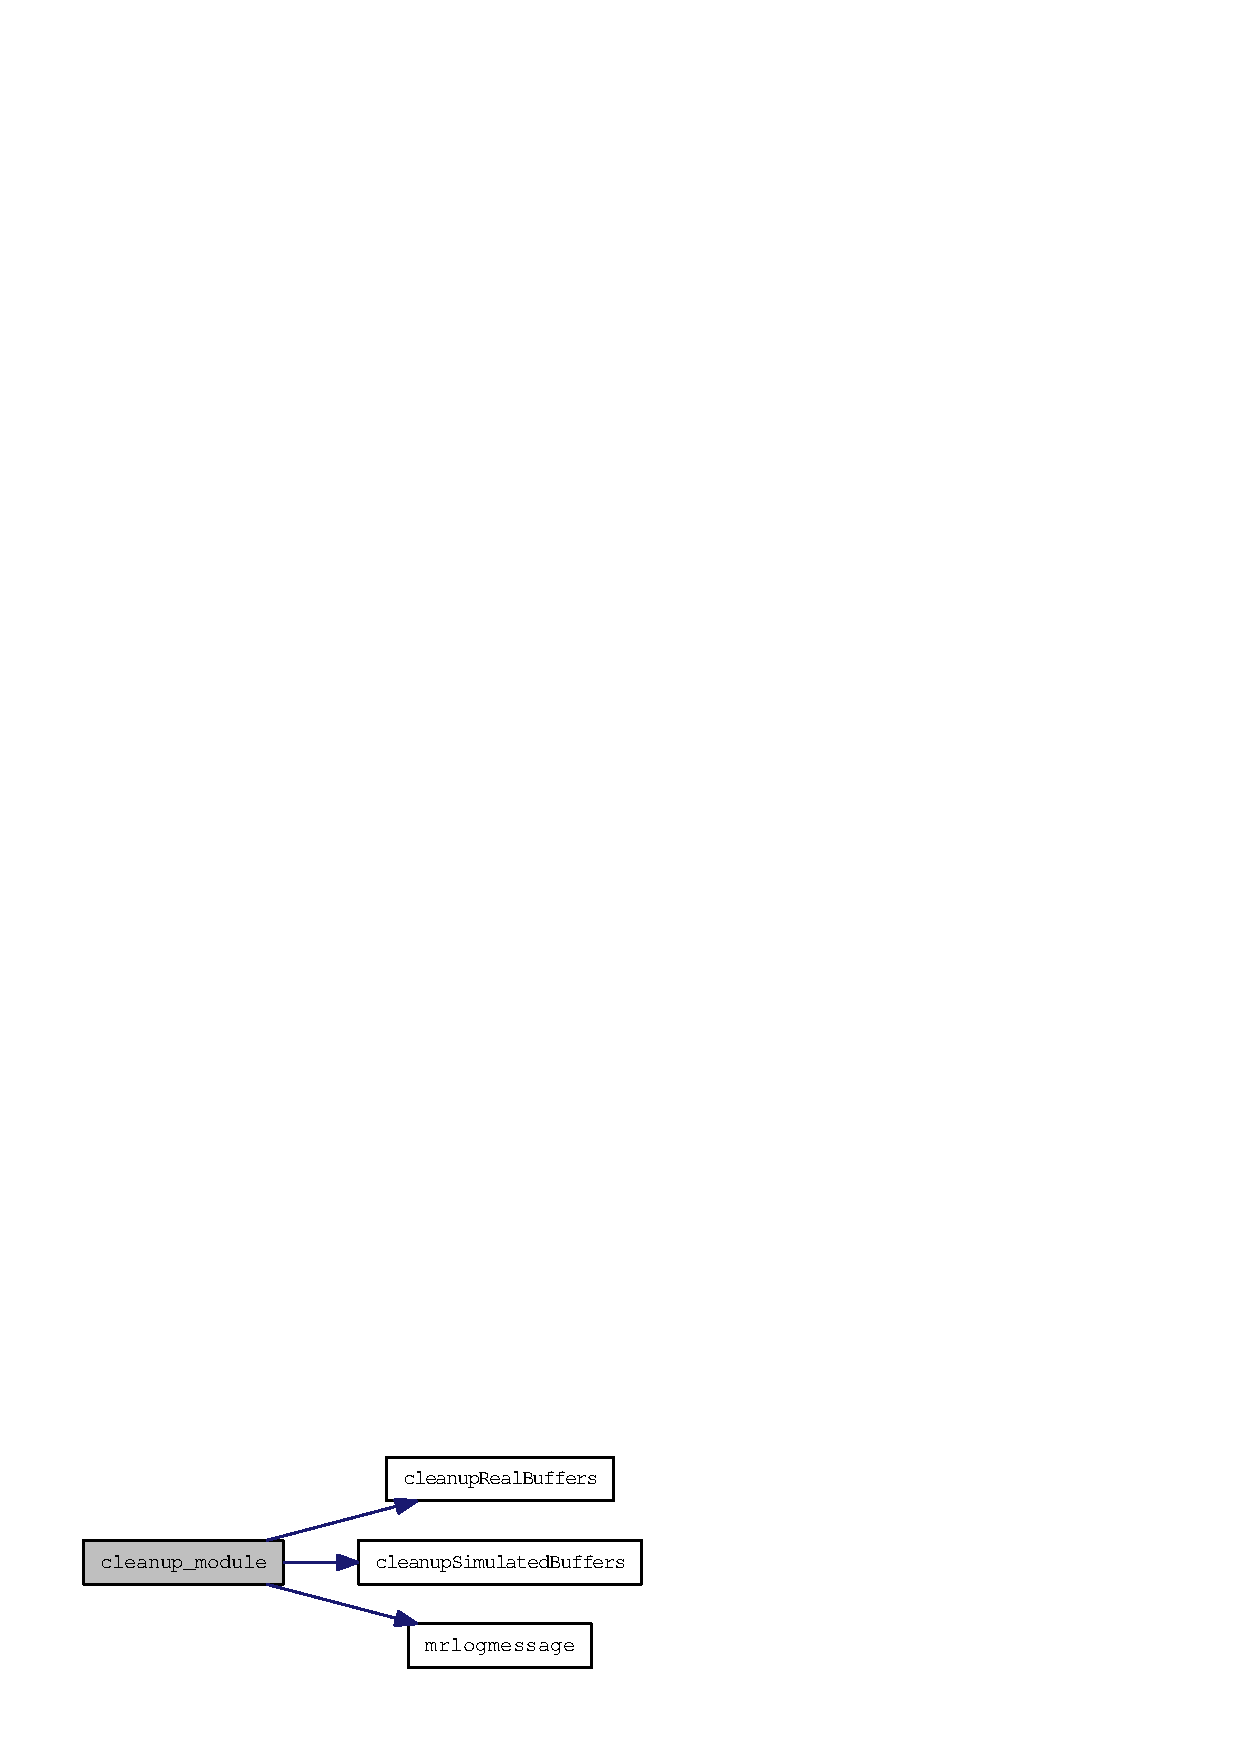
\includegraphics[width=156pt]{backup_2dcs__driver_8c_bb8e1606224e802418862b898888063a_cgraph}
\end{center}
\end{figure}
\hypertarget{backup_2dcs__driver_8c_06a93d1b1348b354639233cdab90e9fe}{
\index{backup/dcs_driver.c@{backup/dcs\_\-driver.c}!cleanupRealBuffers@{cleanupRealBuffers}}
\index{cleanupRealBuffers@{cleanupRealBuffers}!backup/dcs_driver.c@{backup/dcs\_\-driver.c}}
\subsubsection[cleanupRealBuffers]{\setlength{\rightskip}{0pt plus 5cm}void cleanup\-Real\-Buffers ()}}
\label{backup_2dcs__driver_8c_06a93d1b1348b354639233cdab90e9fe}




Definition at line 494 of file backup/dcs\_\-driver.c.

References msgbuf\_\-in\_\-virtbase, msgbuf\_\-out\_\-virtbase, and regfile\_\-virtbase.

Referenced by cleanup\_\-module(), and init\-Real\-Buffers().\hypertarget{backup_2dcs__driver_8c_24611c859ab5512627f0ebe5e71bb7df}{
\index{backup/dcs_driver.c@{backup/dcs\_\-driver.c}!dcs_comparevalue@{dcs\_\-comparevalue}}
\index{dcs_comparevalue@{dcs\_\-comparevalue}!backup/dcs_driver.c@{backup/dcs\_\-driver.c}}
\subsubsection[dcs\_\-comparevalue]{\setlength{\rightskip}{0pt plus 5cm}static int dcs\_\-comparevalue (u32 {\em begin}, u32 {\em size}, u32 {\em value})\hspace{0.3cm}{\tt  \mbox{[}static\mbox{]}}}}
\label{backup_2dcs__driver_8c_24611c859ab5512627f0ebe5e71bb7df}




Definition at line 135 of file backup/dcs\_\-driver.c.

Referenced by init\-Real\-Buffers().\hypertarget{backup_2dcs__driver_8c_85874c4901b4b811c882944a3f77ff0e}{
\index{backup/dcs_driver.c@{backup/dcs\_\-driver.c}!dcs_read@{dcs\_\-read}}
\index{dcs_read@{dcs\_\-read}!backup/dcs_driver.c@{backup/dcs\_\-driver.c}}
\subsubsection[dcs\_\-read]{\setlength{\rightskip}{0pt plus 5cm}static int dcs\_\-read (u32 {\em begin}, u32 {\em size}, u32 $\ast$ {\em buff})\hspace{0.3cm}{\tt  \mbox{[}static\mbox{]}}}}
\label{backup_2dcs__driver_8c_85874c4901b4b811c882944a3f77ff0e}




Definition at line 172 of file backup/dcs\_\-driver.c.

Referenced by dcsc\_\-read().\hypertarget{backup_2dcs__driver_8c_626a935595dad9fb4ce5cfdf4fd48f28}{
\index{backup/dcs_driver.c@{backup/dcs\_\-driver.c}!dcs_write@{dcs\_\-write}}
\index{dcs_write@{dcs\_\-write}!backup/dcs_driver.c@{backup/dcs\_\-driver.c}}
\subsubsection[dcs\_\-write]{\setlength{\rightskip}{0pt plus 5cm}static int dcs\_\-write (u32 {\em begin}, u32 {\em size}, u32 $\ast$ {\em buff})\hspace{0.3cm}{\tt  \mbox{[}static\mbox{]}}}}
\label{backup_2dcs__driver_8c_626a935595dad9fb4ce5cfdf4fd48f28}




Definition at line 197 of file backup/dcs\_\-driver.c.

Referenced by dcsc\_\-write().\hypertarget{backup_2dcs__driver_8c_aec6947dd189feeedeb22af3fbc21d81}{
\index{backup/dcs_driver.c@{backup/dcs\_\-driver.c}!dcs_writevalue@{dcs\_\-writevalue}}
\index{dcs_writevalue@{dcs\_\-writevalue}!backup/dcs_driver.c@{backup/dcs\_\-driver.c}}
\subsubsection[dcs\_\-writevalue]{\setlength{\rightskip}{0pt plus 5cm}static int dcs\_\-writevalue (u32 {\em begin}, u32 {\em size}, u32 {\em value})\hspace{0.3cm}{\tt  \mbox{[}static\mbox{]}}}}
\label{backup_2dcs__driver_8c_aec6947dd189feeedeb22af3fbc21d81}




Definition at line 150 of file backup/dcs\_\-driver.c.

Referenced by init\-Real\-Buffers(), and init\-Simulated\-Buffers().\hypertarget{backup_2dcs__driver_8c_5350bab3f3d6d1f1e2c84ecafa150d68}{
\index{backup/dcs_driver.c@{backup/dcs\_\-driver.c}!dcsc_close@{dcsc\_\-close}}
\index{dcsc_close@{dcsc\_\-close}!backup/dcs_driver.c@{backup/dcs\_\-driver.c}}
\subsubsection[dcsc\_\-close]{\setlength{\rightskip}{0pt plus 5cm}static int dcsc\_\-close (struct inode $\ast$ {\em inode}, struct file $\ast$ {\em filp})\hspace{0.3cm}{\tt  \mbox{[}static\mbox{]}}}}
\label{backup_2dcs__driver_8c_5350bab3f3d6d1f1e2c84ecafa150d68}




Definition at line 840 of file backup/dcs\_\-driver.c.

References LOG\_\-DBG, LOG\_\-OPEN\_\-CLOSE, MR\_\-KERN\_\-DEBUG, and mrlogmessage().

Here is the call graph for this function:\begin{figure}[H]
\begin{center}
\leavevmode
\includegraphics[width=119pt]{backup_2dcs__driver_8c_5350bab3f3d6d1f1e2c84ecafa150d68_cgraph}
\end{center}
\end{figure}
\hypertarget{backup_2dcs__driver_8c_30d7523911ed6cebd68b1d5c34da9d64}{
\index{backup/dcs_driver.c@{backup/dcs\_\-driver.c}!dcsc_ioctl@{dcsc\_\-ioctl}}
\index{dcsc_ioctl@{dcsc\_\-ioctl}!backup/dcs_driver.c@{backup/dcs\_\-driver.c}}
\subsubsection[dcsc\_\-ioctl]{\setlength{\rightskip}{0pt plus 5cm}static int dcsc\_\-ioctl (struct inode $\ast$ {\em inode}, struct file $\ast$ {\em filp}, unsigned int {\em cmd}, unsigned long {\em arg})\hspace{0.3cm}{\tt  \mbox{[}static\mbox{]}}}}
\label{backup_2dcs__driver_8c_30d7523911ed6cebd68b1d5c34da9d64}




Definition at line 854 of file backup/dcs\_\-driver.c.

References dcsc\_\-msgbuf\_\-in\_\-size, dcsc\_\-msgbuf\_\-out\_\-size, dcsc\_\-regfile\_\-size, DRIVER\_\-MAJOR\_\-VERSION\_\-NUMBER, DRIVER\_\-MINOR\_\-VERSION\_\-NUMBER, g\_\-logfilename, g\_\-logflags, IOCTL\_\-ACTIVATE\_\-LOCK, IOCTL\_\-GET\_\-MSGBUF\_\-IN\_\-SIZE, IOCTL\_\-GET\_\-MSGBUF\_\-OUT\_\-SIZE, IOCTL\_\-GET\_\-REGFILE\_\-SIZE, IOCTL\_\-GET\_\-VERS\_\-STR\_\-SIZE, IOCTL\_\-GET\_\-VERSION, IOCTL\_\-GET\_\-VERSION\_\-V02, IOCTL\_\-LOCK\_\-DRIVER, IOCTL\_\-READ\_\-REG, IOCTL\_\-RELEASE\_\-DRIVER, IOCTL\_\-RESET\_\-LOCK, IOCTL\_\-SEIZE\_\-DRIVER, IOCTL\_\-SET\_\-DEBUG\_\-LEVEL, IOCTL\_\-SET\_\-LOG\_\-FILE, IOCTL\_\-TEST\_\-MSGBUF\_\-IN, IOCTL\_\-TEST\_\-MSGBUF\_\-OUT, IOCTL\_\-UNLOCK\_\-DRIVER, IOCTL\_\-WRITE\_\-REG, lock\-Activate(), lock\-Driver(), lock\-Reset(), LOG\_\-DBG, LOG\_\-ERROR, LOG\_\-INFO, LOG\_\-IOCTL, LOG\_\-WARNING, MR\_\-KERN\_\-DEBUG, mrlogmessage(), regfile\_\-virtbase, release\-Driver(), RELEASETYPE, seize\-Driver(), unlock\-Driver(), and VERSION\_\-STRING\_\-SIZE.

Here is the call graph for this function:\begin{figure}[H]
\begin{center}
\leavevmode
\includegraphics[width=292pt]{backup_2dcs__driver_8c_30d7523911ed6cebd68b1d5c34da9d64_cgraph}
\end{center}
\end{figure}
\hypertarget{backup_2dcs__driver_8c_1b18195d839987757d645e7761bdfbc1}{
\index{backup/dcs_driver.c@{backup/dcs\_\-driver.c}!dcsc_llseek@{dcsc\_\-llseek}}
\index{dcsc_llseek@{dcsc\_\-llseek}!backup/dcs_driver.c@{backup/dcs\_\-driver.c}}
\subsubsection[dcsc\_\-llseek]{\setlength{\rightskip}{0pt plus 5cm}static loff\_\-t dcsc\_\-llseek (struct file $\ast$ {\em filp}, loff\_\-t {\em off}, int {\em ref})\hspace{0.3cm}{\tt  \mbox{[}static\mbox{]}}}}
\label{backup_2dcs__driver_8c_1b18195d839987757d645e7761bdfbc1}




Definition at line 675 of file backup/dcs\_\-driver.c.

References LOG\_\-DBG, LOG\_\-ERROR, LOG\_\-LLSEEK, MR\_\-KERN\_\-DEBUG, and mrlogmessage().

Here is the call graph for this function:\begin{figure}[H]
\begin{center}
\leavevmode
\includegraphics[width=120pt]{backup_2dcs__driver_8c_1b18195d839987757d645e7761bdfbc1_cgraph}
\end{center}
\end{figure}
\hypertarget{backup_2dcs__driver_8c_c3b4c74273847bef0006306f638cc133}{
\index{backup/dcs_driver.c@{backup/dcs\_\-driver.c}!dcsc_mmap@{dcsc\_\-mmap}}
\index{dcsc_mmap@{dcsc\_\-mmap}!backup/dcs_driver.c@{backup/dcs\_\-driver.c}}
\subsubsection[dcsc\_\-mmap]{\setlength{\rightskip}{0pt plus 5cm}static int dcsc\_\-mmap (struct file $\ast$ {\em filp}, struct vm\_\-area\_\-struct $\ast$ {\em vma})\hspace{0.3cm}{\tt  \mbox{[}static\mbox{]}}}}
\label{backup_2dcs__driver_8c_c3b4c74273847bef0006306f638cc133}




Definition at line 847 of file backup/dcs\_\-driver.c.

References LOG\_\-DBG, LOG\_\-MMAP, MR\_\-KERN\_\-DEBUG, and mrlogmessage().

Here is the call graph for this function:\begin{figure}[H]
\begin{center}
\leavevmode
\includegraphics[width=122pt]{backup_2dcs__driver_8c_c3b4c74273847bef0006306f638cc133_cgraph}
\end{center}
\end{figure}
\hypertarget{backup_2dcs__driver_8c_1fc34702f88baf2a47a0434f6ea9e0cb}{
\index{backup/dcs_driver.c@{backup/dcs\_\-driver.c}!dcsc_open@{dcsc\_\-open}}
\index{dcsc_open@{dcsc\_\-open}!backup/dcs_driver.c@{backup/dcs\_\-driver.c}}
\subsubsection[dcsc\_\-open]{\setlength{\rightskip}{0pt plus 5cm}static int dcsc\_\-open (struct inode $\ast$ {\em inode}, struct file $\ast$ {\em filp})\hspace{0.3cm}{\tt  \mbox{[}static\mbox{]}}}}
\label{backup_2dcs__driver_8c_1fc34702f88baf2a47a0434f6ea9e0cb}




Definition at line 825 of file backup/dcs\_\-driver.c.

References dcsc\_\-msgbuf\_\-in\_\-size, dcsc\_\-msgbuf\_\-out\_\-size, dcsc\_\-regfile\_\-size, LOG\_\-ERROR, LOG\_\-INFO, LOG\_\-OPEN\_\-CLOSE, MR\_\-KERN\_\-DEBUG, mrlogmessage(), msgbuf\_\-in\_\-virtbase, msgbuf\_\-out\_\-virtbase, and regfile\_\-virtbase.

Here is the call graph for this function:\begin{figure}[H]
\begin{center}
\leavevmode
\includegraphics[width=119pt]{backup_2dcs__driver_8c_1fc34702f88baf2a47a0434f6ea9e0cb_cgraph}
\end{center}
\end{figure}
\hypertarget{backup_2dcs__driver_8c_8067a5efccbb89b363e4b12d4249bb07}{
\index{backup/dcs_driver.c@{backup/dcs\_\-driver.c}!dcsc_read@{dcsc\_\-read}}
\index{dcsc_read@{dcsc\_\-read}!backup/dcs_driver.c@{backup/dcs\_\-driver.c}}
\subsubsection[dcsc\_\-read]{\setlength{\rightskip}{0pt plus 5cm}static int dcsc\_\-read (struct file $\ast$ {\em filp}, char $\ast$ {\em buf}, size\_\-t {\em count}, loff\_\-t $\ast$ {\em f\_\-pos})\hspace{0.3cm}{\tt  \mbox{[}static\mbox{]}}}}
\label{backup_2dcs__driver_8c_8067a5efccbb89b363e4b12d4249bb07}




Definition at line 690 of file backup/dcs\_\-driver.c.

References ACCESS\_\-ALL, dcs\_\-read(), dcsc\_\-msgbuf\_\-in\_\-size, dcsc\_\-msgbuf\_\-out\_\-size, dcsc\_\-regfile\_\-size, i\-Access\-Mode, LOG\_\-DBG, LOG\_\-ERROR, LOG\_\-READ\_\-WRITE, LOG\_\-WARNING, MR\_\-KERN\_\-DEBUG, mrlogmessage(), msgbuf\_\-in\_\-virtbase, msgbuf\_\-out\_\-virtbase, and regfile\_\-virtbase.

Here is the call graph for this function:\begin{figure}[H]
\begin{center}
\leavevmode
\includegraphics[width=117pt]{backup_2dcs__driver_8c_8067a5efccbb89b363e4b12d4249bb07_cgraph}
\end{center}
\end{figure}
\hypertarget{backup_2dcs__driver_8c_0c28bf0d1a698b2c9c598715bd37a9cb}{
\index{backup/dcs_driver.c@{backup/dcs\_\-driver.c}!dcsc_write@{dcsc\_\-write}}
\index{dcsc_write@{dcsc\_\-write}!backup/dcs_driver.c@{backup/dcs\_\-driver.c}}
\subsubsection[dcsc\_\-write]{\setlength{\rightskip}{0pt plus 5cm}static int dcsc\_\-write (struct file $\ast$ {\em filp}, const char $\ast$ {\em buf}, size\_\-t {\em count}, loff\_\-t $\ast$ {\em f\_\-pos})\hspace{0.3cm}{\tt  \mbox{[}static\mbox{]}}}}
\label{backup_2dcs__driver_8c_0c28bf0d1a698b2c9c598715bd37a9cb}




Definition at line 759 of file backup/dcs\_\-driver.c.

References ACCESS\_\-ALL, dcs\_\-write(), dcsc\_\-msgbuf\_\-in\_\-size, dcsc\_\-msgbuf\_\-out\_\-size, dcsc\_\-regfile\_\-size, i\-Access\-Mode, LOG\_\-DBG, LOG\_\-ERROR, LOG\_\-READ\_\-WRITE, LOG\_\-WARNING, MR\_\-KERN\_\-DEBUG, mrlogmessage(), msgbuf\_\-in\_\-virtbase, msgbuf\_\-out\_\-virtbase, and regfile\_\-virtbase.

Here is the call graph for this function:\begin{figure}[H]
\begin{center}
\leavevmode
\includegraphics[width=118pt]{backup_2dcs__driver_8c_0c28bf0d1a698b2c9c598715bd37a9cb_cgraph}
\end{center}
\end{figure}
\hypertarget{backup_2dcs__driver_8c_0f2edb55399fbd36008bbded20c5ecab}{
\index{backup/dcs_driver.c@{backup/dcs\_\-driver.c}!findBufferForAddress@{findBufferForAddress}}
\index{findBufferForAddress@{findBufferForAddress}!backup/dcs_driver.c@{backup/dcs\_\-driver.c}}
\subsubsection[findBufferForAddress]{\setlength{\rightskip}{0pt plus 5cm}u32 find\-Buffer\-For\-Address (loff\_\-t {\em offset}, int {\em i\-Access\-Mode}, u32 $\ast$$\ast$ {\em pp\-Buffer}, u32 $\ast$ {\em p\-Position}, const char $\ast$$\ast$ {\em pp\-Buffer\-Name})}}
\label{backup_2dcs__driver_8c_0f2edb55399fbd36008bbded20c5ecab}




Definition at line 225 of file backup/dcs\_\-driver.c.

References ACCESS\_\-IN\_\-BUFFER, ACCESS\_\-OUT\_\-BUFFER, ACCESS\_\-REGFILE, dcsc\_\-msgbuf\_\-in\_\-size, dcsc\_\-msgbuf\_\-out\_\-size, dcsc\_\-regfile\_\-size, LOG\_\-FLAG\_\-ALL, mrlogmessage(), msgbuf\_\-in\_\-virtbase, msgbuf\_\-out\_\-virtbase, and regfile\_\-virtbase.

Here is the call graph for this function:\begin{figure}[H]
\begin{center}
\leavevmode
\includegraphics[width=143pt]{backup_2dcs__driver_8c_0f2edb55399fbd36008bbded20c5ecab_cgraph}
\end{center}
\end{figure}
\hypertarget{backup_2dcs__driver_8c_e52690ce6969b799366b2c5feba67b8c}{
\index{backup/dcs_driver.c@{backup/dcs\_\-driver.c}!init_module@{init\_\-module}}
\index{init_module@{init\_\-module}!backup/dcs_driver.c@{backup/dcs\_\-driver.c}}
\subsubsection[init\_\-module]{\setlength{\rightskip}{0pt plus 5cm}int init\_\-module (void)}}
\label{backup_2dcs__driver_8c_e52690ce6969b799366b2c5feba67b8c}




Definition at line 624 of file backup/dcs\_\-driver.c.

References dcsc\_\-fops, dcsc\_\-major\-ID, DRIVER\_\-MAJOR\_\-VERSION\_\-NUMBER, DRIVER\_\-MINOR\_\-VERSION\_\-NUMBER, Init\-Driver\-Lock(), init\-Real\-Buffers(), LOG\_\-ERROR, LOG\_\-INFO, mrlogmessage(), and RELEASETYPE.

Here is the call graph for this function:\begin{figure}[H]
\begin{center}
\leavevmode
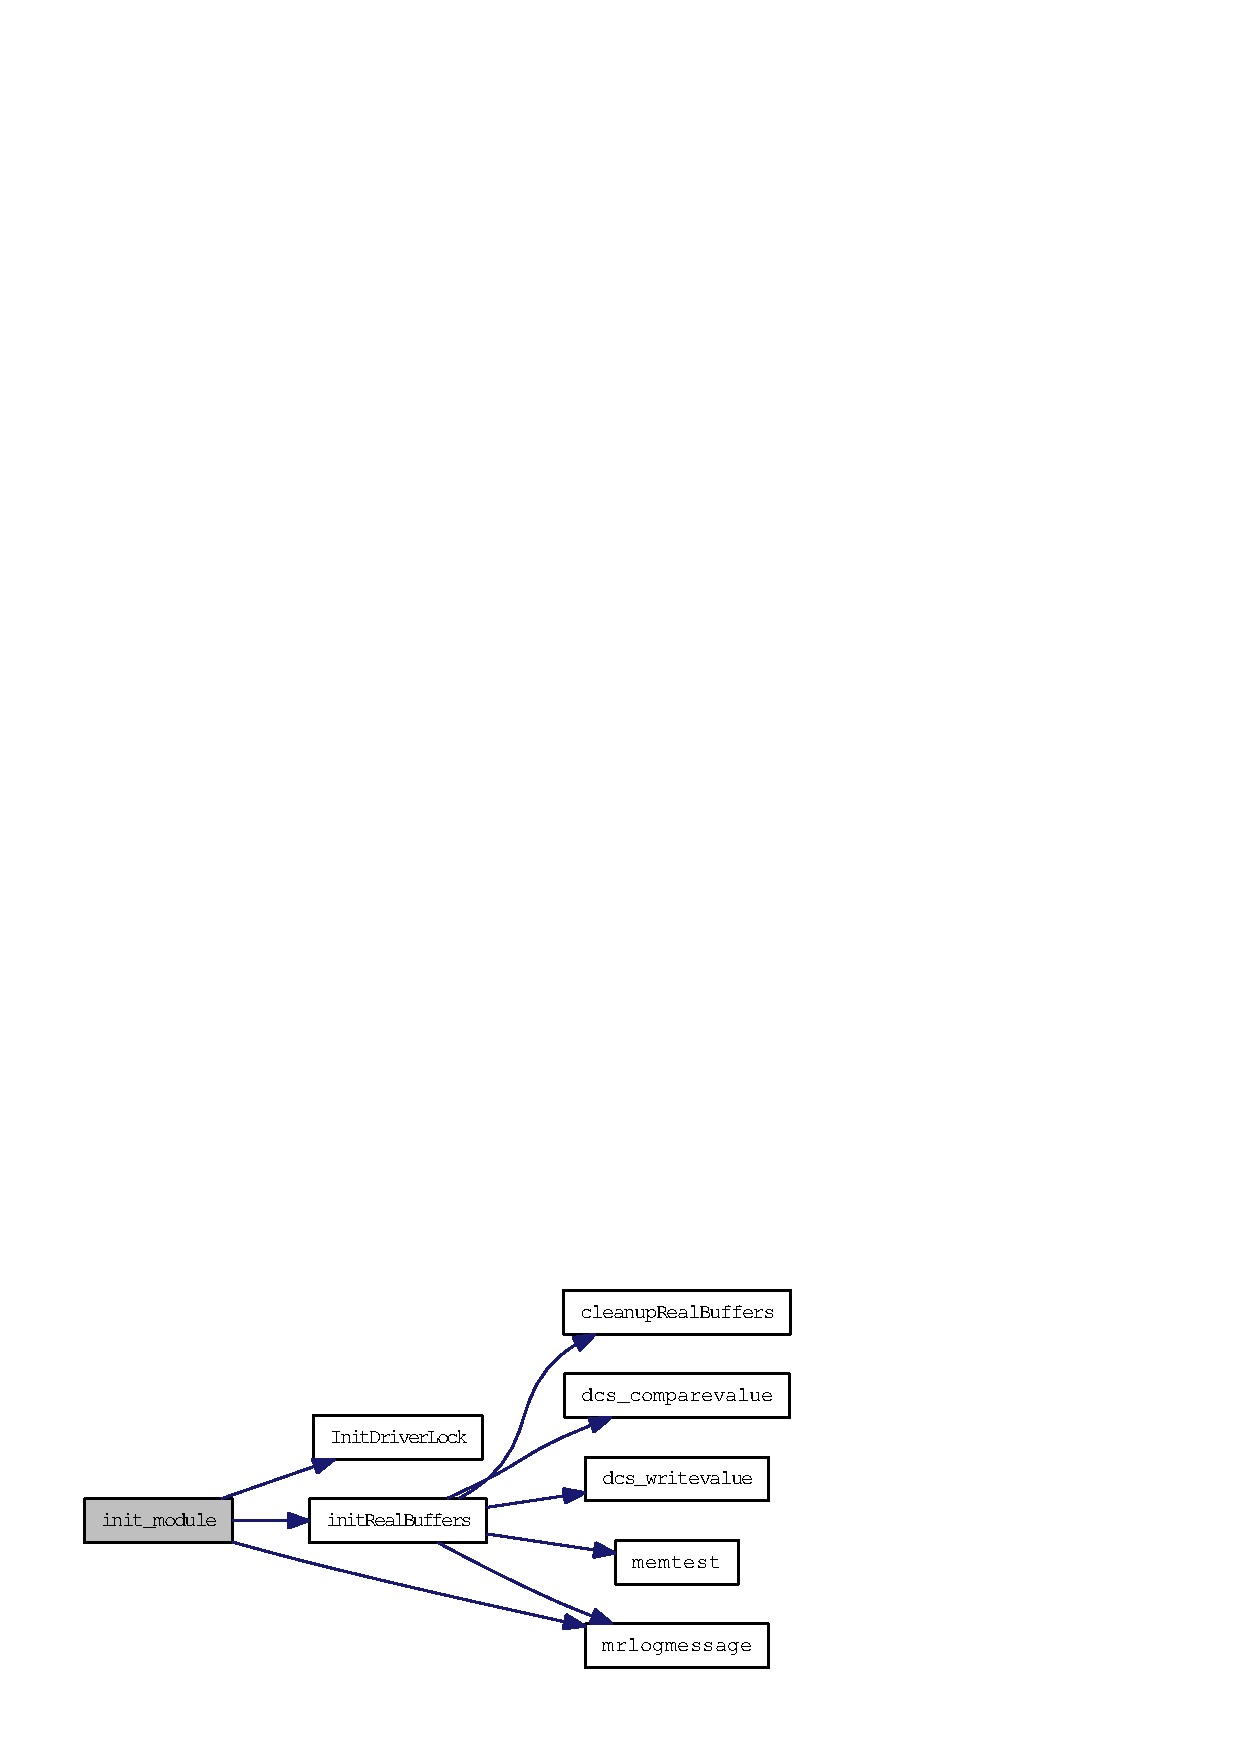
\includegraphics[width=192pt]{backup_2dcs__driver_8c_e52690ce6969b799366b2c5feba67b8c_cgraph}
\end{center}
\end{figure}
\hypertarget{backup_2dcs__driver_8c_c619293d4edc146efb03fb6b03f8461f}{
\index{backup/dcs_driver.c@{backup/dcs\_\-driver.c}!InitDriverLock@{InitDriverLock}}
\index{InitDriverLock@{InitDriverLock}!backup/dcs_driver.c@{backup/dcs\_\-driver.c}}
\subsubsection[InitDriverLock]{\setlength{\rightskip}{0pt plus 5cm}int Init\-Driver\-Lock (void)}}
\label{backup_2dcs__driver_8c_c619293d4edc146efb03fb6b03f8461f}




Definition at line 289 of file backup/dcs\_\-driver.c.

References g\_\-i\-Lock, g\_\-i\-Lock\-Initialized, g\_\-i\-Lock\-Pid, g\_\-i\-Lock\-Reset, g\_\-i\-Seize\-Code, g\_\-spinlock, and g\_\-wait\-Queue.

Referenced by init\_\-module().\hypertarget{backup_2dcs__driver_8c_b3161c882ef5359bf75cf6705c545cd4}{
\index{backup/dcs_driver.c@{backup/dcs\_\-driver.c}!initRealBuffers@{initRealBuffers}}
\index{initRealBuffers@{initRealBuffers}!backup/dcs_driver.c@{backup/dcs\_\-driver.c}}
\subsubsection[initRealBuffers]{\setlength{\rightskip}{0pt plus 5cm}int init\-Real\-Buffers ()}}
\label{backup_2dcs__driver_8c_b3161c882ef5359bf75cf6705c545cd4}




Definition at line 505 of file backup/dcs\_\-driver.c.

References cleanup\-Real\-Buffers(), dcs\_\-comparevalue(), dcs\_\-writevalue(), dcsc\_\-msgbuf\_\-in\_\-size, dcsc\_\-msgbuf\_\-out\_\-size, dcsc\_\-regfile\_\-size, LOG\_\-DBG, LOG\_\-ERROR, LOG\_\-INTERNAL, memtest(), MR\_\-KERN\_\-DEBUG, mrlogmessage(), msgbuf\_\-in\_\-physaddr, msgbuf\_\-in\_\-virtbase, msgbuf\_\-out\_\-physaddr, msgbuf\_\-out\_\-virtbase, regfile\_\-physaddr, regfile\_\-virtbase, and TEST\_\-PATTERN.

Referenced by init\_\-module().

Here is the call graph for this function:\begin{figure}[H]
\begin{center}
\leavevmode
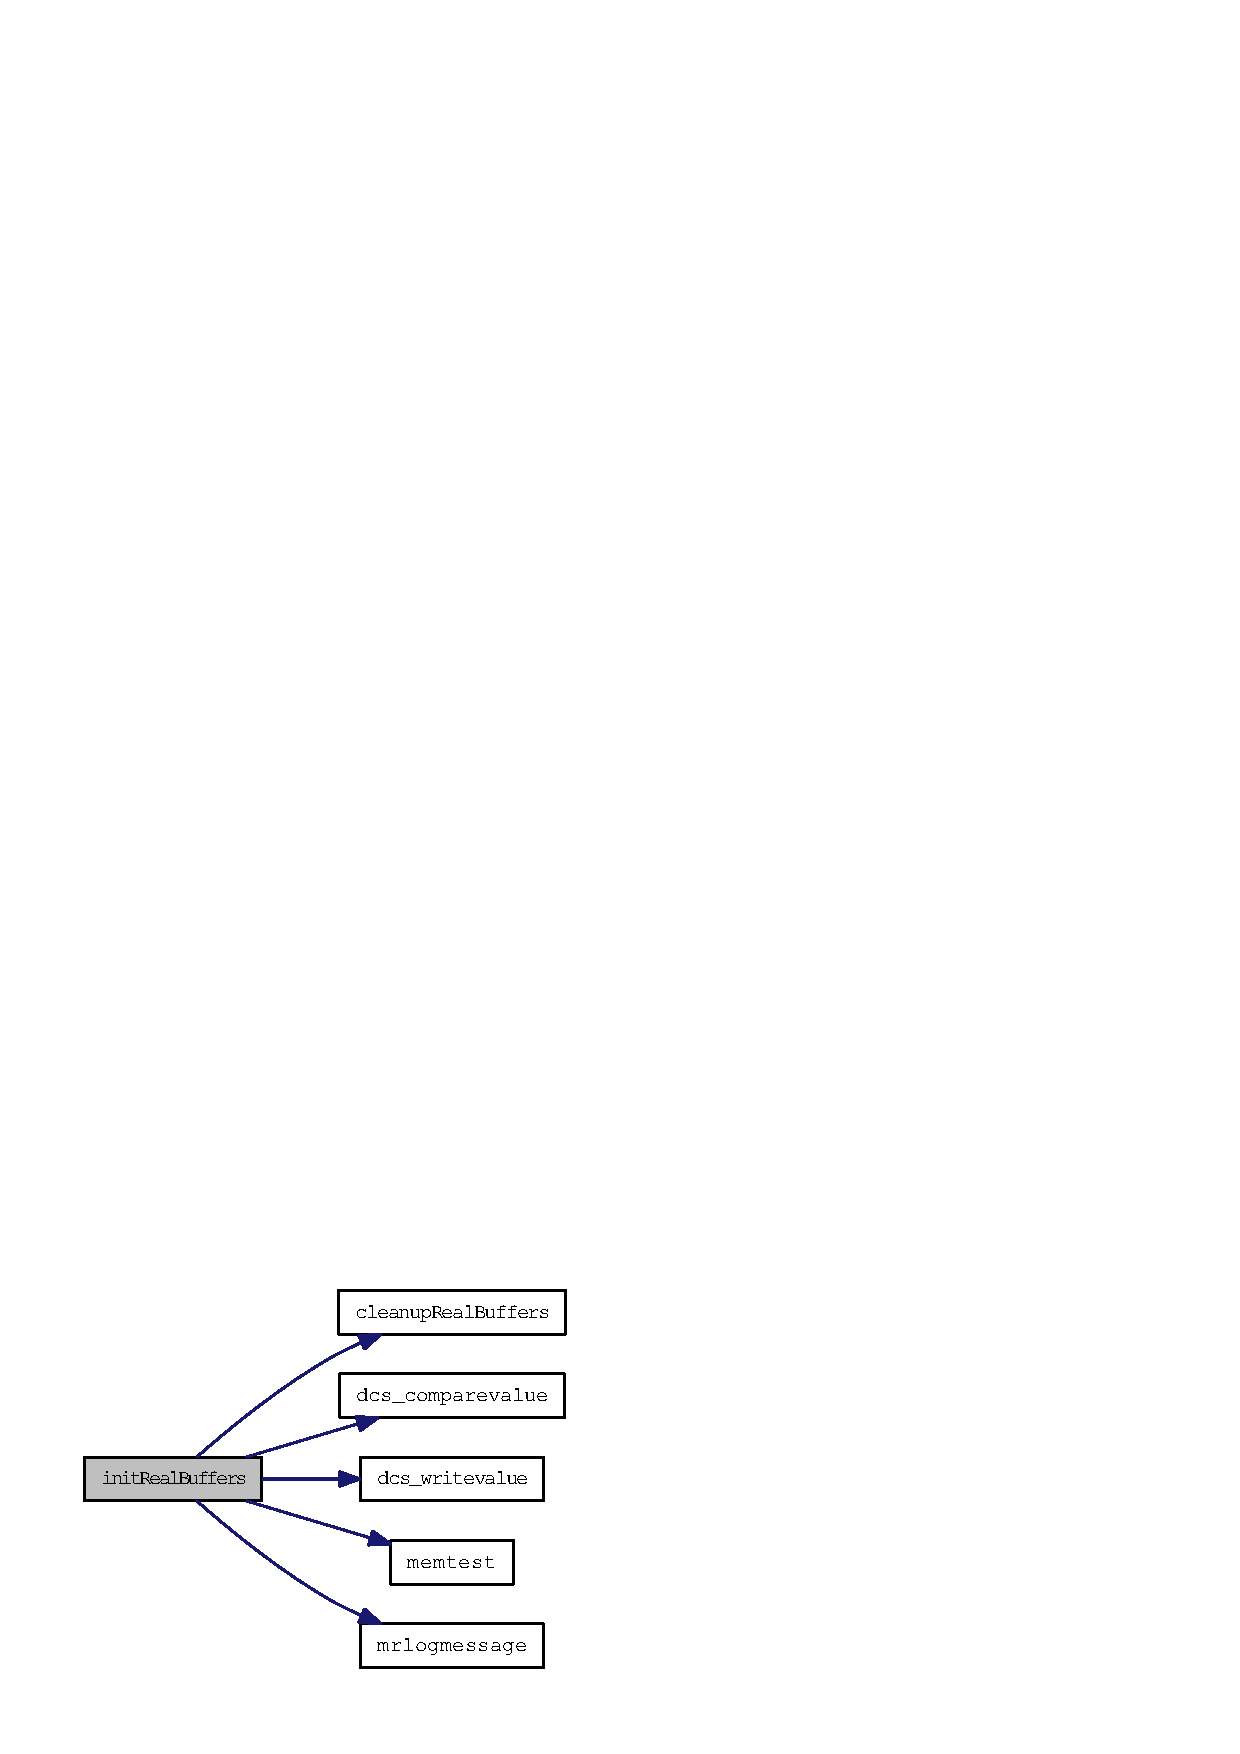
\includegraphics[width=138pt]{backup_2dcs__driver_8c_b3161c882ef5359bf75cf6705c545cd4_cgraph}
\end{center}
\end{figure}
\hypertarget{backup_2dcs__driver_8c_a754eaa169b47cb26cf5e997276ebd81}{
\index{backup/dcs_driver.c@{backup/dcs\_\-driver.c}!lockActivate@{lockActivate}}
\index{lockActivate@{lockActivate}!backup/dcs_driver.c@{backup/dcs\_\-driver.c}}
\subsubsection[lockActivate]{\setlength{\rightskip}{0pt plus 5cm}int lock\-Activate (void)}}
\label{backup_2dcs__driver_8c_a754eaa169b47cb26cf5e997276ebd81}




Definition at line 302 of file backup/dcs\_\-driver.c.

References g\_\-i\-Lock\-Reset.

Referenced by dcsc\_\-ioctl().\hypertarget{backup_2dcs__driver_8c_69f4b1ea76e4eeed7eb2fed3adc6e847}{
\index{backup/dcs_driver.c@{backup/dcs\_\-driver.c}!lockDriver@{lockDriver}}
\index{lockDriver@{lockDriver}!backup/dcs_driver.c@{backup/dcs\_\-driver.c}}
\subsubsection[lockDriver]{\setlength{\rightskip}{0pt plus 5cm}int lock\-Driver (int {\em i\-Seize\-Code}, int {\em i\-Time\-Out})}}
\label{backup_2dcs__driver_8c_69f4b1ea76e4eeed7eb2fed3adc6e847}


Try to lock the driver, go to sleep if already locked. 

After the process got woken up it tries again to lock. \begin{Desc}
\item[Parameters:]
\begin{description}
\item[{\em i\-Seize\-Code}]master lock code given by the application \item[{\em i\-Time\-Out}]time out (currently not used) \end{description}
\end{Desc}
\begin{Desc}
\item[Returns:]1 if free and now set, 0 if already blocked\par
 -ETIMEDOUT if time out\par
 -EPERM driver in master lock \end{Desc}


Definition at line 363 of file backup/dcs\_\-driver.c.

References check\-And\-Lock(), g\_\-i\-Lock\-Initialized, g\_\-i\-Lock\-Reset, g\_\-wait\-Queue, LOG\_\-DBG, LOG\_\-DRIVER\_\-LCK, MR\_\-KERN\_\-DEBUG, and mrlogmessage().

Referenced by dcsc\_\-ioctl(), release\-Driver(), and seize\-Driver().

Here is the call graph for this function:\begin{figure}[H]
\begin{center}
\leavevmode
\includegraphics[width=178pt]{backup_2dcs__driver_8c_69f4b1ea76e4eeed7eb2fed3adc6e847_cgraph}
\end{center}
\end{figure}
\hypertarget{backup_2dcs__driver_8c_bfe7c9dd41295bc3fe20fc96aa3ac39d}{
\index{backup/dcs_driver.c@{backup/dcs\_\-driver.c}!lockReset@{lockReset}}
\index{lockReset@{lockReset}!backup/dcs_driver.c@{backup/dcs\_\-driver.c}}
\subsubsection[lockReset]{\setlength{\rightskip}{0pt plus 5cm}int lock\-Reset (void)}}
\label{backup_2dcs__driver_8c_bfe7c9dd41295bc3fe20fc96aa3ac39d}




Definition at line 309 of file backup/dcs\_\-driver.c.

References g\_\-i\-Lock, g\_\-i\-Lock\-Initialized, g\_\-i\-Lock\-Pid, g\_\-i\-Lock\-Reset, g\_\-i\-Seize\-Code, and g\_\-wait\-Queue.

Referenced by dcsc\_\-ioctl().\hypertarget{backup_2dcs__driver_8c_5fc9e61f41c571cca4373a64ca28d159}{
\index{backup/dcs_driver.c@{backup/dcs\_\-driver.c}!memtest@{memtest}}
\index{memtest@{memtest}!backup/dcs_driver.c@{backup/dcs\_\-driver.c}}
\subsubsection[memtest]{\setlength{\rightskip}{0pt plus 5cm}static int memtest (u32 {\em begin}, u32 {\em size})\hspace{0.3cm}{\tt  \mbox{[}static\mbox{]}}}}
\label{backup_2dcs__driver_8c_5fc9e61f41c571cca4373a64ca28d159}




Definition at line 113 of file backup/dcs\_\-driver.c.

Referenced by init\-Real\-Buffers(), and init\-Simulated\-Buffers().\hypertarget{backup_2dcs__driver_8c_53fff30413e173391c35bdc5481c1719}{
\index{backup/dcs_driver.c@{backup/dcs\_\-driver.c}!MODULE_AUTHOR@{MODULE\_\-AUTHOR}}
\index{MODULE_AUTHOR@{MODULE\_\-AUTHOR}!backup/dcs_driver.c@{backup/dcs\_\-driver.c}}
\subsubsection[MODULE\_\-AUTHOR]{\setlength{\rightskip}{0pt plus 5cm}MODULE\_\-AUTHOR (\char`\"{}Matthias Richter\char`\"{})}}
\label{backup_2dcs__driver_8c_53fff30413e173391c35bdc5481c1719}


\hypertarget{backup_2dcs__driver_8c_2eb38dffd9d03b7908c57b56ae9e9377}{
\index{backup/dcs_driver.c@{backup/dcs\_\-driver.c}!MODULE_DESCRIPTION@{MODULE\_\-DESCRIPTION}}
\index{MODULE_DESCRIPTION@{MODULE\_\-DESCRIPTION}!backup/dcs_driver.c@{backup/dcs\_\-driver.c}}
\subsubsection[MODULE\_\-DESCRIPTION]{\setlength{\rightskip}{0pt plus 5cm}MODULE\_\-DESCRIPTION (\char`\"{}dcs-card register driver\char`\"{})}}
\label{backup_2dcs__driver_8c_2eb38dffd9d03b7908c57b56ae9e9377}


\hypertarget{backup_2dcs__driver_8c_d94b36675e7eb067ea3ce6ff9e244a44}{
\index{backup/dcs_driver.c@{backup/dcs\_\-driver.c}!MODULE_LICENSE@{MODULE\_\-LICENSE}}
\index{MODULE_LICENSE@{MODULE\_\-LICENSE}!backup/dcs_driver.c@{backup/dcs\_\-driver.c}}
\subsubsection[MODULE\_\-LICENSE]{\setlength{\rightskip}{0pt plus 5cm}MODULE\_\-LICENSE (\char`\"{}GPL\char`\"{})}}
\label{backup_2dcs__driver_8c_d94b36675e7eb067ea3ce6ff9e244a44}


\hypertarget{backup_2dcs__driver_8c_84a8ddb935ced6da7bdd97965f36cead}{
\index{backup/dcs_driver.c@{backup/dcs\_\-driver.c}!MODULE_PARM@{MODULE\_\-PARM}}
\index{MODULE_PARM@{MODULE\_\-PARM}!backup/dcs_driver.c@{backup/dcs\_\-driver.c}}
\subsubsection[MODULE\_\-PARM]{\setlength{\rightskip}{0pt plus 5cm}MODULE\_\-PARM (\hyperlink{dcs__driver_8c_607a6fb1f19bf1e11ec4fa99dc7efecd}{regfile\_\-physaddr}, \char`\"{}i\char`\"{})}}
\label{backup_2dcs__driver_8c_84a8ddb935ced6da7bdd97965f36cead}


\hypertarget{backup_2dcs__driver_8c_b8f38a668f504ecdbf2041c14fc8f50f}{
\index{backup/dcs_driver.c@{backup/dcs\_\-driver.c}!MODULE_PARM@{MODULE\_\-PARM}}
\index{MODULE_PARM@{MODULE\_\-PARM}!backup/dcs_driver.c@{backup/dcs\_\-driver.c}}
\subsubsection[MODULE\_\-PARM]{\setlength{\rightskip}{0pt plus 5cm}MODULE\_\-PARM (\hyperlink{dcs__driver_8c_89c68fc835da1b91e1d93eecb77922b6}{msgbuf\_\-out\_\-physaddr}, \char`\"{}i\char`\"{})}}
\label{backup_2dcs__driver_8c_b8f38a668f504ecdbf2041c14fc8f50f}


\hypertarget{backup_2dcs__driver_8c_73936caf0f944aa65a75a16e077c835a}{
\index{backup/dcs_driver.c@{backup/dcs\_\-driver.c}!MODULE_PARM@{MODULE\_\-PARM}}
\index{MODULE_PARM@{MODULE\_\-PARM}!backup/dcs_driver.c@{backup/dcs\_\-driver.c}}
\subsubsection[MODULE\_\-PARM]{\setlength{\rightskip}{0pt plus 5cm}MODULE\_\-PARM (\hyperlink{dcs__driver_8c_03af36d4209f6364a9f7a5f1087f19f9}{msgbuf\_\-in\_\-physaddr}, \char`\"{}i\char`\"{})}}
\label{backup_2dcs__driver_8c_73936caf0f944aa65a75a16e077c835a}


\hypertarget{backup_2dcs__driver_8c_19e37b390f71b35e88960d78c6d836c4}{
\index{backup/dcs_driver.c@{backup/dcs\_\-driver.c}!MODULE_PARM@{MODULE\_\-PARM}}
\index{MODULE_PARM@{MODULE\_\-PARM}!backup/dcs_driver.c@{backup/dcs\_\-driver.c}}
\subsubsection[MODULE\_\-PARM]{\setlength{\rightskip}{0pt plus 5cm}MODULE\_\-PARM (\hyperlink{dcs__driver_8c_898ab396bb466832c0c38ecc37f16632}{dcsc\_\-regfile\_\-size}, \char`\"{}i\char`\"{})}}
\label{backup_2dcs__driver_8c_19e37b390f71b35e88960d78c6d836c4}


\hypertarget{backup_2dcs__driver_8c_d2a9008a63b5fc661f4aa83a8a0f8bcc}{
\index{backup/dcs_driver.c@{backup/dcs\_\-driver.c}!MODULE_PARM@{MODULE\_\-PARM}}
\index{MODULE_PARM@{MODULE\_\-PARM}!backup/dcs_driver.c@{backup/dcs\_\-driver.c}}
\subsubsection[MODULE\_\-PARM]{\setlength{\rightskip}{0pt plus 5cm}MODULE\_\-PARM (\hyperlink{dcs__driver_8c_57243357aaca143dc0a0e93dcd16eb89}{dcsc\_\-msgbuf\_\-out\_\-size}, \char`\"{}i\char`\"{})}}
\label{backup_2dcs__driver_8c_d2a9008a63b5fc661f4aa83a8a0f8bcc}


\hypertarget{backup_2dcs__driver_8c_75f25d27ddf2830f44e578fb39146b97}{
\index{backup/dcs_driver.c@{backup/dcs\_\-driver.c}!MODULE_PARM@{MODULE\_\-PARM}}
\index{MODULE_PARM@{MODULE\_\-PARM}!backup/dcs_driver.c@{backup/dcs\_\-driver.c}}
\subsubsection[MODULE\_\-PARM]{\setlength{\rightskip}{0pt plus 5cm}MODULE\_\-PARM (\hyperlink{dcs__driver_8c_9a8b5688625d4564010909cb4e23192f}{dcsc\_\-msgbuf\_\-in\_\-size}, \char`\"{}i\char`\"{})}}
\label{backup_2dcs__driver_8c_75f25d27ddf2830f44e578fb39146b97}


\hypertarget{backup_2dcs__driver_8c_3053a7067223a09a392be7f5871f9766}{
\index{backup/dcs_driver.c@{backup/dcs\_\-driver.c}!MODULE_PARM@{MODULE\_\-PARM}}
\index{MODULE_PARM@{MODULE\_\-PARM}!backup/dcs_driver.c@{backup/dcs\_\-driver.c}}
\subsubsection[MODULE\_\-PARM]{\setlength{\rightskip}{0pt plus 5cm}MODULE\_\-PARM (\hyperlink{dcs__driver_8c_45c631d40e14d14a309abbe2b87ccd1b}{dcsc\_\-major\-ID}, \char`\"{}i\char`\"{})}}
\label{backup_2dcs__driver_8c_3053a7067223a09a392be7f5871f9766}


\hypertarget{backup_2dcs__driver_8c_6ccbabe02e6e0af40d2b653b2a158d40}{
\index{backup/dcs_driver.c@{backup/dcs\_\-driver.c}!releaseDriver@{releaseDriver}}
\index{releaseDriver@{releaseDriver}!backup/dcs_driver.c@{backup/dcs\_\-driver.c}}
\subsubsection[releaseDriver]{\setlength{\rightskip}{0pt plus 5cm}int release\-Driver (int {\em i\-Seize\-Code})}}
\label{backup_2dcs__driver_8c_6ccbabe02e6e0af40d2b653b2a158d40}


Release the driver which was locked to a single application. 

The is the pendant to \hyperlink{dcs__driver_8c_f65c837b7c30c1d6c4861e5dbb9a4e59}{seize\-Driver}. \begin{Desc}
\item[Parameters:]
\begin{description}
\item[{\em i\-Seize\-Code}]master lock code given by the application \end{description}
\end{Desc}
\begin{Desc}
\item[Returns:]$>$=0 if success, neg. error code if failed \end{Desc}


Definition at line 441 of file backup/dcs\_\-driver.c.

References g\_\-i\-Seize\-Code, lock\-Driver(), LOG\_\-DRIVER\_\-LCK, LOG\_\-ERROR, LOG\_\-INFO, mrlogmessage(), and unlock\-Driver().

Referenced by dcsc\_\-ioctl().

Here is the call graph for this function:\begin{figure}[H]
\begin{center}
\leavevmode
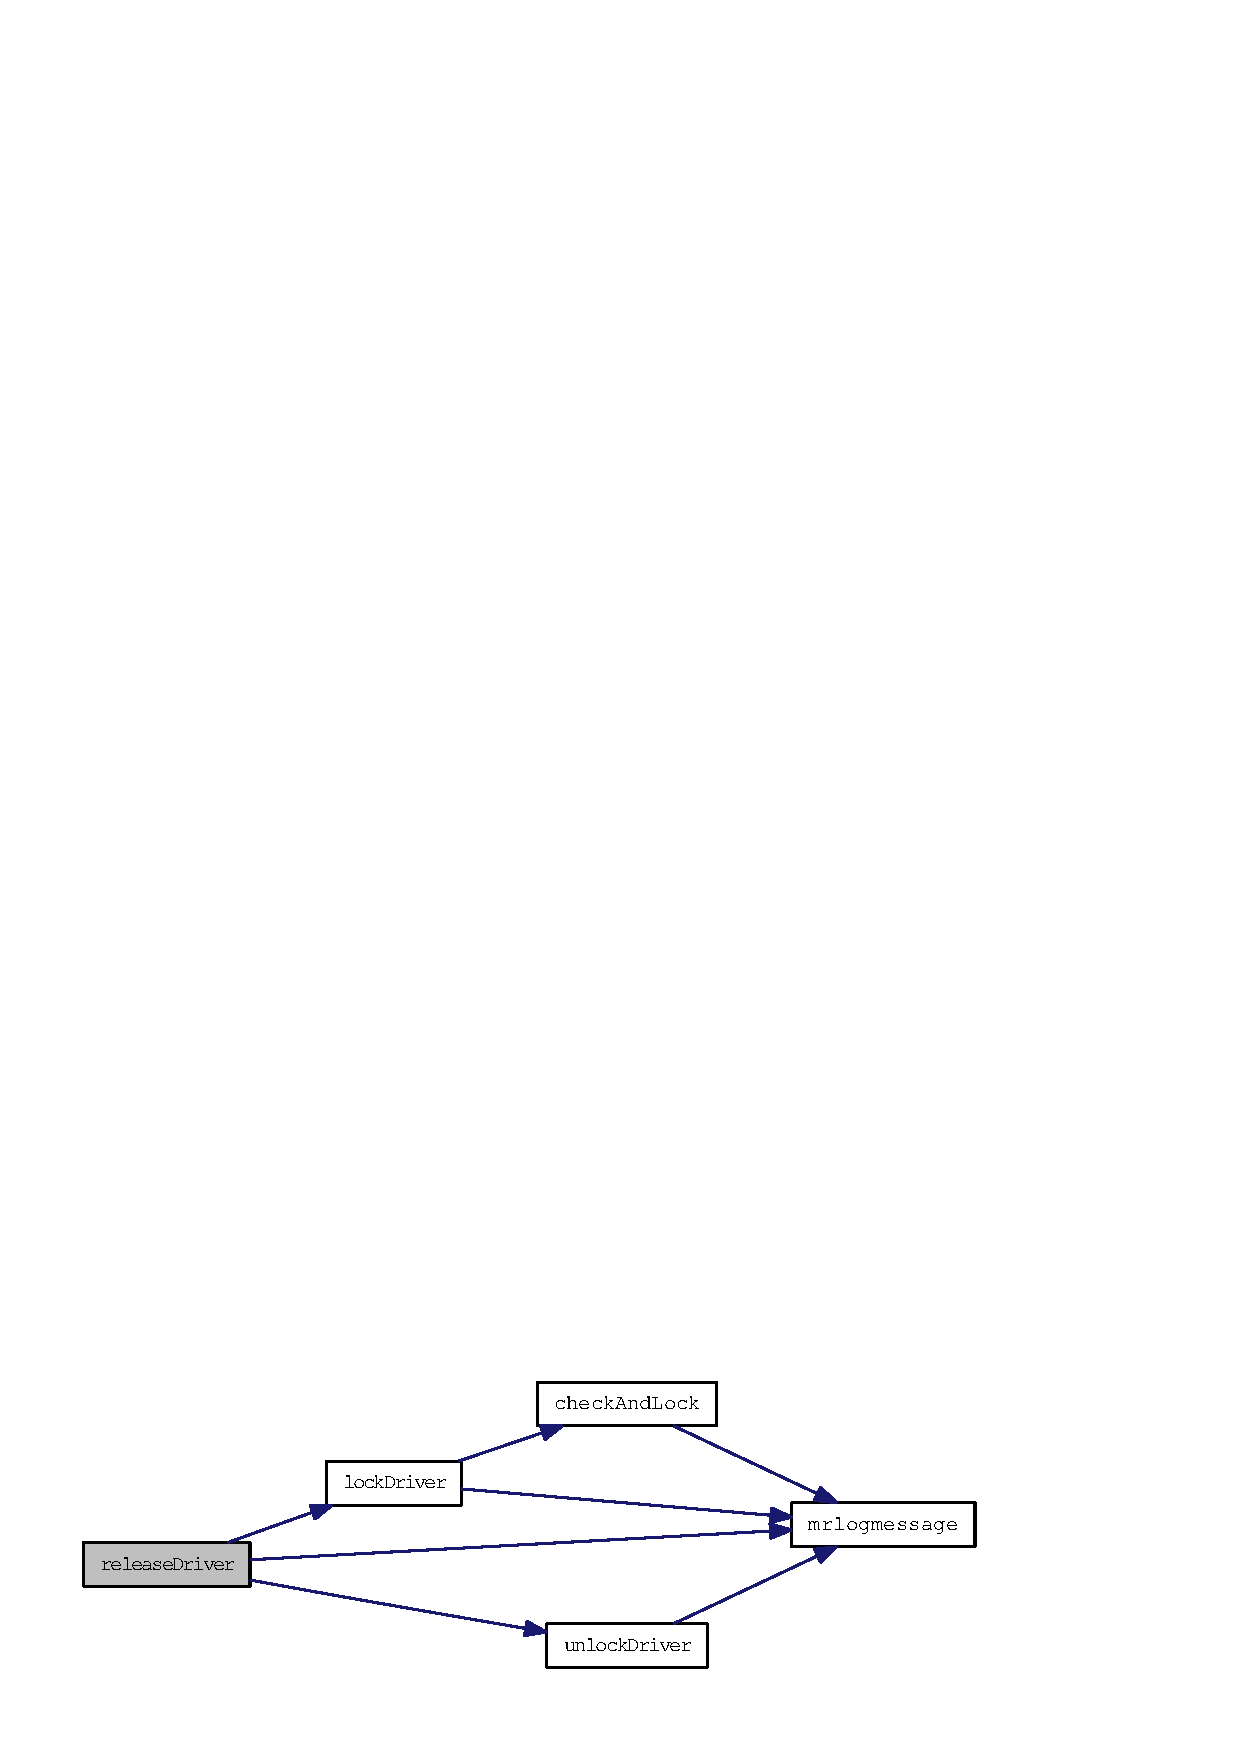
\includegraphics[width=236pt]{backup_2dcs__driver_8c_6ccbabe02e6e0af40d2b653b2a158d40_cgraph}
\end{center}
\end{figure}
\hypertarget{backup_2dcs__driver_8c_f65c837b7c30c1d6c4861e5dbb9a4e59}{
\index{backup/dcs_driver.c@{backup/dcs\_\-driver.c}!seizeDriver@{seizeDriver}}
\index{seizeDriver@{seizeDriver}!backup/dcs_driver.c@{backup/dcs\_\-driver.c}}
\subsubsection[seizeDriver]{\setlength{\rightskip}{0pt plus 5cm}int seize\-Driver (int {\em i\-Seize\-Code})}}
\label{backup_2dcs__driver_8c_f65c837b7c30c1d6c4861e5dbb9a4e59}


Lock the driver to a single application. 

The normal lock works for the different treads of that application, but no other application has the right to access. \begin{Desc}
\item[Parameters:]
\begin{description}
\item[{\em i\-Seize\-Code}]a code to identify the master application \end{description}
\end{Desc}
\begin{Desc}
\item[Returns:]$>$=0 if success, neg. error code if failed\par
 -EPERM driver seized by another application \end{Desc}


Definition at line 389 of file backup/dcs\_\-driver.c.

References g\_\-i\-Seize\-Code, lock\-Driver(), LOG\_\-DRIVER\_\-LCK, LOG\_\-ERROR, LOG\_\-INFO, LOG\_\-WARNING, mrlogmessage(), and unlock\-Driver().

Referenced by dcsc\_\-ioctl().

Here is the call graph for this function:\begin{figure}[H]
\begin{center}
\leavevmode
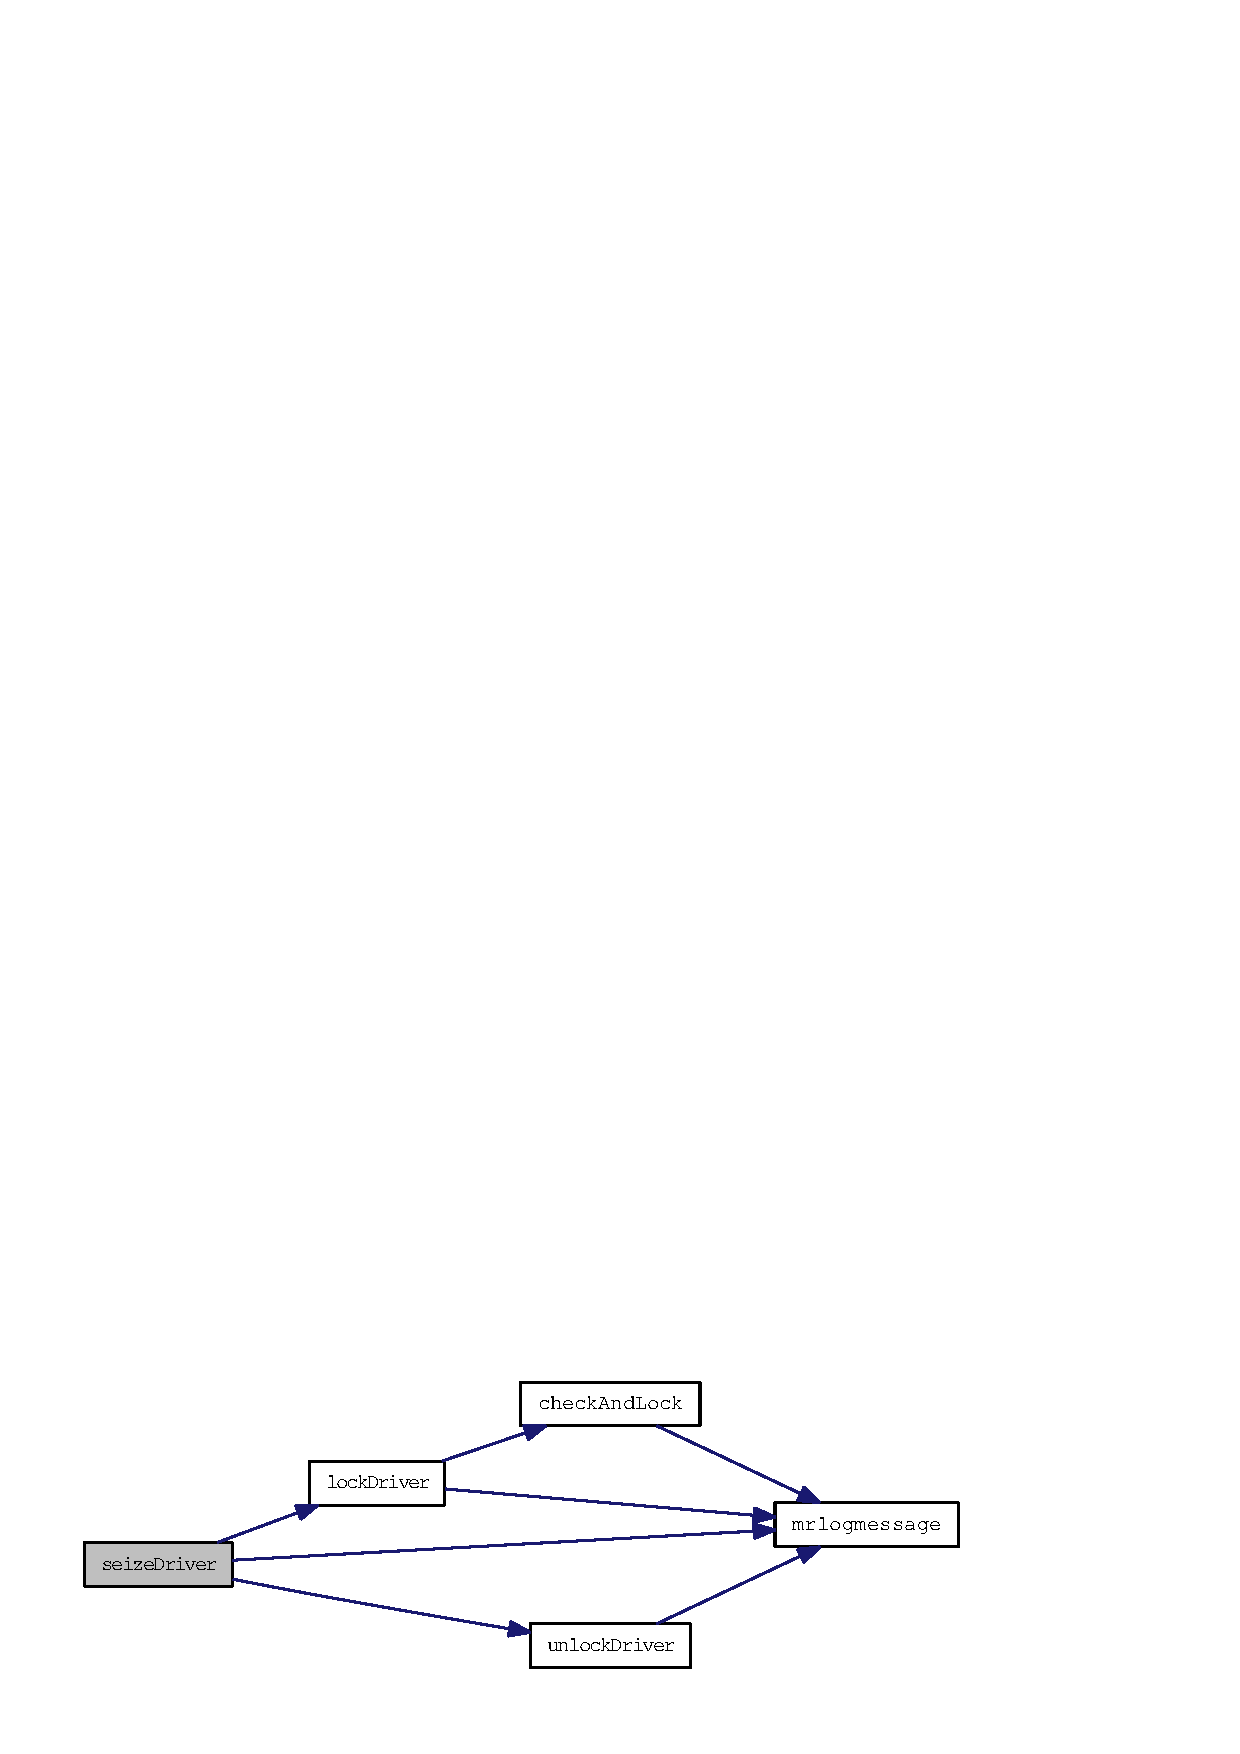
\includegraphics[width=232pt]{backup_2dcs__driver_8c_f65c837b7c30c1d6c4861e5dbb9a4e59_cgraph}
\end{center}
\end{figure}
\hypertarget{backup_2dcs__driver_8c_0e119609dea51ec090e7852dd9d0abad}{
\index{backup/dcs_driver.c@{backup/dcs\_\-driver.c}!unlockDriver@{unlockDriver}}
\index{unlockDriver@{unlockDriver}!backup/dcs_driver.c@{backup/dcs\_\-driver.c}}
\subsubsection[unlockDriver]{\setlength{\rightskip}{0pt plus 5cm}int unlock\-Driver (void)}}
\label{backup_2dcs__driver_8c_0e119609dea51ec090e7852dd9d0abad}


Unlock the driver and wake up all sleeping processes. 



Definition at line 410 of file backup/dcs\_\-driver.c.

References g\_\-i\-Lock, g\_\-i\-Lock\-Initialized, g\_\-i\-Lock\-Pid, g\_\-spinlock, g\_\-wait\-Queue, LOG\_\-DBG, LOG\_\-DRIVER\_\-LCK, LOG\_\-ERROR, LOG\_\-WARNING, MR\_\-KERN\_\-DEBUG, and mrlogmessage().

Referenced by dcsc\_\-ioctl(), release\-Driver(), and seize\-Driver().

Here is the call graph for this function:\begin{figure}[H]
\begin{center}
\leavevmode
\includegraphics[width=123pt]{backup_2dcs__driver_8c_0e119609dea51ec090e7852dd9d0abad_cgraph}
\end{center}
\end{figure}


\subsection{Variable Documentation}
\hypertarget{backup_2dcs__driver_8c_010266ee96b0e2fd685de9f760d64dd8}{
\index{backup/dcs_driver.c@{backup/dcs\_\-driver.c}!dcsc_fops@{dcsc\_\-fops}}
\index{dcsc_fops@{dcsc\_\-fops}!backup/dcs_driver.c@{backup/dcs\_\-driver.c}}
\subsubsection[dcsc\_\-fops]{\setlength{\rightskip}{0pt plus 5cm}struct file\_\-operations \hyperlink{dcs__driver_8c_010266ee96b0e2fd685de9f760d64dd8}{dcsc\_\-fops}}}
\label{backup_2dcs__driver_8c_010266ee96b0e2fd685de9f760d64dd8}


\textbf{Initial value:}

\begin{Code}\begin{verbatim} {
  llseek:  dcsc_llseek,
  read:    dcsc_read,
  write:   dcsc_write,
  ioctl:   dcsc_ioctl,
  mmap:    dcsc_mmap,
  open:    dcsc_open,
  release: dcsc_close,
}
\end{verbatim}\end{Code}


Definition at line 480 of file backup/dcs\_\-driver.c.

Referenced by init\_\-module().\hypertarget{backup_2dcs__driver_8c_45c631d40e14d14a309abbe2b87ccd1b}{
\index{backup/dcs_driver.c@{backup/dcs\_\-driver.c}!dcsc_majorID@{dcsc\_\-majorID}}
\index{dcsc_majorID@{dcsc\_\-majorID}!backup/dcs_driver.c@{backup/dcs\_\-driver.c}}
\subsubsection[dcsc\_\-majorID]{\setlength{\rightskip}{0pt plus 5cm}int \hyperlink{dcs__driver_8c_45c631d40e14d14a309abbe2b87ccd1b}{dcsc\_\-major\-ID} = 150}}
\label{backup_2dcs__driver_8c_45c631d40e14d14a309abbe2b87ccd1b}




Definition at line 49 of file backup/dcs\_\-driver.c.

Referenced by cleanup\_\-module(), and init\_\-module().\hypertarget{backup_2dcs__driver_8c_9a8b5688625d4564010909cb4e23192f}{
\index{backup/dcs_driver.c@{backup/dcs\_\-driver.c}!dcsc_msgbuf_in_size@{dcsc\_\-msgbuf\_\-in\_\-size}}
\index{dcsc_msgbuf_in_size@{dcsc\_\-msgbuf\_\-in\_\-size}!backup/dcs_driver.c@{backup/dcs\_\-driver.c}}
\subsubsection[dcsc\_\-msgbuf\_\-in\_\-size]{\setlength{\rightskip}{0pt plus 5cm}int \hyperlink{dcs__driver_8c_9a8b5688625d4564010909cb4e23192f}{dcsc\_\-msgbuf\_\-in\_\-size} = 0x400\hspace{0.3cm}{\tt  \mbox{[}static\mbox{]}}}}
\label{backup_2dcs__driver_8c_9a8b5688625d4564010909cb4e23192f}




Definition at line 71 of file backup/dcs\_\-driver.c.

Referenced by dcsc\_\-ioctl(), dcsc\_\-open(), dcsc\_\-read(), dcsc\_\-write(), find\-Buffer\-For\-Address(), init\-Real\-Buffers(), and init\-Simulated\-Buffers().\hypertarget{backup_2dcs__driver_8c_57243357aaca143dc0a0e93dcd16eb89}{
\index{backup/dcs_driver.c@{backup/dcs\_\-driver.c}!dcsc_msgbuf_out_size@{dcsc\_\-msgbuf\_\-out\_\-size}}
\index{dcsc_msgbuf_out_size@{dcsc\_\-msgbuf\_\-out\_\-size}!backup/dcs_driver.c@{backup/dcs\_\-driver.c}}
\subsubsection[dcsc\_\-msgbuf\_\-out\_\-size]{\setlength{\rightskip}{0pt plus 5cm}int \hyperlink{dcs__driver_8c_57243357aaca143dc0a0e93dcd16eb89}{dcsc\_\-msgbuf\_\-out\_\-size} = 0x400\hspace{0.3cm}{\tt  \mbox{[}static\mbox{]}}}}
\label{backup_2dcs__driver_8c_57243357aaca143dc0a0e93dcd16eb89}




Definition at line 72 of file backup/dcs\_\-driver.c.

Referenced by dcsc\_\-ioctl(), dcsc\_\-open(), dcsc\_\-read(), dcsc\_\-write(), find\-Buffer\-For\-Address(), init\-Real\-Buffers(), and init\-Simulated\-Buffers().\hypertarget{backup_2dcs__driver_8c_898ab396bb466832c0c38ecc37f16632}{
\index{backup/dcs_driver.c@{backup/dcs\_\-driver.c}!dcsc_regfile_size@{dcsc\_\-regfile\_\-size}}
\index{dcsc_regfile_size@{dcsc\_\-regfile\_\-size}!backup/dcs_driver.c@{backup/dcs\_\-driver.c}}
\subsubsection[dcsc\_\-regfile\_\-size]{\setlength{\rightskip}{0pt plus 5cm}int \hyperlink{dcs__driver_8c_898ab396bb466832c0c38ecc37f16632}{dcsc\_\-regfile\_\-size} = 0x10\hspace{0.3cm}{\tt  \mbox{[}static\mbox{]}}}}
\label{backup_2dcs__driver_8c_898ab396bb466832c0c38ecc37f16632}




Definition at line 73 of file backup/dcs\_\-driver.c.

Referenced by dcsc\_\-ioctl(), dcsc\_\-open(), dcsc\_\-read(), dcsc\_\-write(), find\-Buffer\-For\-Address(), init\-Real\-Buffers(), and init\-Simulated\-Buffers().\hypertarget{backup_2dcs__driver_8c_18b5596c6309017456c046d61b05e3b1}{
\index{backup/dcs_driver.c@{backup/dcs\_\-driver.c}!g_iLock@{g\_\-iLock}}
\index{g_iLock@{g\_\-iLock}!backup/dcs_driver.c@{backup/dcs\_\-driver.c}}
\subsubsection[g\_\-iLock]{\setlength{\rightskip}{0pt plus 5cm}int \hyperlink{dcs__driver_8c_18b5596c6309017456c046d61b05e3b1}{g\_\-i\-Lock} = 0}}
\label{backup_2dcs__driver_8c_18b5596c6309017456c046d61b05e3b1}




Definition at line 283 of file backup/dcs\_\-driver.c.

Referenced by check\-And\-Lock(), Init\-Driver\-Lock(), lock\-Reset(), and unlock\-Driver().\hypertarget{backup_2dcs__driver_8c_c23aa679017a305c1a149016fea0c003}{
\index{backup/dcs_driver.c@{backup/dcs\_\-driver.c}!g_iLockInitialized@{g\_\-iLockInitialized}}
\index{g_iLockInitialized@{g\_\-iLockInitialized}!backup/dcs_driver.c@{backup/dcs\_\-driver.c}}
\subsubsection[g\_\-iLockInitialized]{\setlength{\rightskip}{0pt plus 5cm}int \hyperlink{dcs__driver_8c_c23aa679017a305c1a149016fea0c003}{g\_\-i\-Lock\-Initialized} = 0}}
\label{backup_2dcs__driver_8c_c23aa679017a305c1a149016fea0c003}




Definition at line 287 of file backup/dcs\_\-driver.c.

Referenced by check\-And\-Lock(), Init\-Driver\-Lock(), lock\-Driver(), lock\-Reset(), and unlock\-Driver().\hypertarget{backup_2dcs__driver_8c_750fd6e08c92777b860f11e575a4e804}{
\index{backup/dcs_driver.c@{backup/dcs\_\-driver.c}!g_iLockPid@{g\_\-iLockPid}}
\index{g_iLockPid@{g\_\-iLockPid}!backup/dcs_driver.c@{backup/dcs\_\-driver.c}}
\subsubsection[g\_\-iLockPid]{\setlength{\rightskip}{0pt plus 5cm}int \hyperlink{dcs__driver_8c_750fd6e08c92777b860f11e575a4e804}{g\_\-i\-Lock\-Pid} = 0}}
\label{backup_2dcs__driver_8c_750fd6e08c92777b860f11e575a4e804}




Definition at line 284 of file backup/dcs\_\-driver.c.

Referenced by check\-And\-Lock(), Init\-Driver\-Lock(), lock\-Reset(), and unlock\-Driver().\hypertarget{backup_2dcs__driver_8c_983d0af3572a91f1c34b942ff8954544}{
\index{backup/dcs_driver.c@{backup/dcs\_\-driver.c}!g_iLockReset@{g\_\-iLockReset}}
\index{g_iLockReset@{g\_\-iLockReset}!backup/dcs_driver.c@{backup/dcs\_\-driver.c}}
\subsubsection[g\_\-iLockReset]{\setlength{\rightskip}{0pt plus 5cm}int \hyperlink{dcs__driver_8c_983d0af3572a91f1c34b942ff8954544}{g\_\-i\-Lock\-Reset} = 0}}
\label{backup_2dcs__driver_8c_983d0af3572a91f1c34b942ff8954544}




Definition at line 282 of file backup/dcs\_\-driver.c.

Referenced by Init\-Driver\-Lock(), lock\-Activate(), lock\-Driver(), and lock\-Reset().\hypertarget{backup_2dcs__driver_8c_2d3bbc70ca9389e34e840e3c3fade06d}{
\index{backup/dcs_driver.c@{backup/dcs\_\-driver.c}!g_iSeizeCode@{g\_\-iSeizeCode}}
\index{g_iSeizeCode@{g\_\-iSeizeCode}!backup/dcs_driver.c@{backup/dcs\_\-driver.c}}
\subsubsection[g\_\-iSeizeCode]{\setlength{\rightskip}{0pt plus 5cm}int \hyperlink{dcs__driver_8c_2d3bbc70ca9389e34e840e3c3fade06d}{g\_\-i\-Seize\-Code} = 0}}
\label{backup_2dcs__driver_8c_2d3bbc70ca9389e34e840e3c3fade06d}




Definition at line 285 of file backup/dcs\_\-driver.c.

Referenced by check\-And\-Lock(), Init\-Driver\-Lock(), lock\-Reset(), release\-Driver(), and seize\-Driver().\hypertarget{backup_2dcs__driver_8c_2f3f72c4a42056343b2c0ac401326cb4}{
\index{backup/dcs_driver.c@{backup/dcs\_\-driver.c}!g_spinlock@{g\_\-spinlock}}
\index{g_spinlock@{g\_\-spinlock}!backup/dcs_driver.c@{backup/dcs\_\-driver.c}}
\subsubsection[g\_\-spinlock]{\setlength{\rightskip}{0pt plus 5cm}spinlock\_\-t \hyperlink{dcs__driver_8c_2f3f72c4a42056343b2c0ac401326cb4}{g\_\-spinlock}}}
\label{backup_2dcs__driver_8c_2f3f72c4a42056343b2c0ac401326cb4}




Definition at line 286 of file backup/dcs\_\-driver.c.

Referenced by check\-And\-Lock(), Init\-Driver\-Lock(), and unlock\-Driver().\hypertarget{backup_2dcs__driver_8c_c5ac2769997c4ac1e8307c4521c4b20e}{
\index{backup/dcs_driver.c@{backup/dcs\_\-driver.c}!g_waitQueue@{g\_\-waitQueue}}
\index{g_waitQueue@{g\_\-waitQueue}!backup/dcs_driver.c@{backup/dcs\_\-driver.c}}
\subsubsection[g\_\-waitQueue]{\setlength{\rightskip}{0pt plus 5cm}wait\_\-queue\_\-head\_\-t \hyperlink{dcs__driver_8c_c5ac2769997c4ac1e8307c4521c4b20e}{g\_\-wait\-Queue}}}
\label{backup_2dcs__driver_8c_c5ac2769997c4ac1e8307c4521c4b20e}




Definition at line 281 of file backup/dcs\_\-driver.c.

Referenced by Init\-Driver\-Lock(), lock\-Driver(), lock\-Reset(), and unlock\-Driver().\hypertarget{backup_2dcs__driver_8c_269775bb092dfa3a11844c3d1883d988}{
\index{backup/dcs_driver.c@{backup/dcs\_\-driver.c}!iAccessMode@{iAccessMode}}
\index{iAccessMode@{iAccessMode}!backup/dcs_driver.c@{backup/dcs\_\-driver.c}}
\subsubsection[iAccessMode]{\setlength{\rightskip}{0pt plus 5cm}int \hyperlink{dcs__driver_8c_269775bb092dfa3a11844c3d1883d988}{i\-Access\-Mode} = ACCESS\_\-ALL\hspace{0.3cm}{\tt  \mbox{[}static\mbox{]}}}}
\label{backup_2dcs__driver_8c_269775bb092dfa3a11844c3d1883d988}




Definition at line 102 of file backup/dcs\_\-driver.c.

Referenced by dcsc\_\-read(), and dcsc\_\-write().\hypertarget{backup_2dcs__driver_8c_03af36d4209f6364a9f7a5f1087f19f9}{
\index{backup/dcs_driver.c@{backup/dcs\_\-driver.c}!msgbuf_in_physaddr@{msgbuf\_\-in\_\-physaddr}}
\index{msgbuf_in_physaddr@{msgbuf\_\-in\_\-physaddr}!backup/dcs_driver.c@{backup/dcs\_\-driver.c}}
\subsubsection[msgbuf\_\-in\_\-physaddr]{\setlength{\rightskip}{0pt plus 5cm}u32$\ast$ \hyperlink{dcs__driver_8c_03af36d4209f6364a9f7a5f1087f19f9}{msgbuf\_\-in\_\-physaddr} = ((u32 $\ast$) 0x80000400)\hspace{0.3cm}{\tt  \mbox{[}static\mbox{]}}}}
\label{backup_2dcs__driver_8c_03af36d4209f6364a9f7a5f1087f19f9}




Definition at line 74 of file backup/dcs\_\-driver.c.

Referenced by init\-Real\-Buffers().\hypertarget{backup_2dcs__driver_8c_a6f29aaef9f61f455e1eeb2890ca8300}{
\index{backup/dcs_driver.c@{backup/dcs\_\-driver.c}!msgbuf_in_virtbase@{msgbuf\_\-in\_\-virtbase}}
\index{msgbuf_in_virtbase@{msgbuf\_\-in\_\-virtbase}!backup/dcs_driver.c@{backup/dcs\_\-driver.c}}
\subsubsection[msgbuf\_\-in\_\-virtbase]{\setlength{\rightskip}{0pt plus 5cm}u32$\ast$ \hyperlink{dcs__driver_8c_a6f29aaef9f61f455e1eeb2890ca8300}{msgbuf\_\-in\_\-virtbase} = NULL\hspace{0.3cm}{\tt  \mbox{[}static\mbox{]}}}}
\label{backup_2dcs__driver_8c_a6f29aaef9f61f455e1eeb2890ca8300}




Definition at line 79 of file backup/dcs\_\-driver.c.

Referenced by cleanup\-Real\-Buffers(), dcsc\_\-open(), dcsc\_\-read(), dcsc\_\-write(), find\-Buffer\-For\-Address(), and init\-Real\-Buffers().\hypertarget{backup_2dcs__driver_8c_89c68fc835da1b91e1d93eecb77922b6}{
\index{backup/dcs_driver.c@{backup/dcs\_\-driver.c}!msgbuf_out_physaddr@{msgbuf\_\-out\_\-physaddr}}
\index{msgbuf_out_physaddr@{msgbuf\_\-out\_\-physaddr}!backup/dcs_driver.c@{backup/dcs\_\-driver.c}}
\subsubsection[msgbuf\_\-out\_\-physaddr]{\setlength{\rightskip}{0pt plus 5cm}u32$\ast$ \hyperlink{dcs__driver_8c_89c68fc835da1b91e1d93eecb77922b6}{msgbuf\_\-out\_\-physaddr} = ((u32 $\ast$) 0x80000800)\hspace{0.3cm}{\tt  \mbox{[}static\mbox{]}}}}
\label{backup_2dcs__driver_8c_89c68fc835da1b91e1d93eecb77922b6}




Definition at line 75 of file backup/dcs\_\-driver.c.

Referenced by init\-Real\-Buffers().\hypertarget{backup_2dcs__driver_8c_6bd1f1592c9416c2bb4de131829a232d}{
\index{backup/dcs_driver.c@{backup/dcs\_\-driver.c}!msgbuf_out_virtbase@{msgbuf\_\-out\_\-virtbase}}
\index{msgbuf_out_virtbase@{msgbuf\_\-out\_\-virtbase}!backup/dcs_driver.c@{backup/dcs\_\-driver.c}}
\subsubsection[msgbuf\_\-out\_\-virtbase]{\setlength{\rightskip}{0pt plus 5cm}u32$\ast$ \hyperlink{dcs__driver_8c_6bd1f1592c9416c2bb4de131829a232d}{msgbuf\_\-out\_\-virtbase} = NULL\hspace{0.3cm}{\tt  \mbox{[}static\mbox{]}}}}
\label{backup_2dcs__driver_8c_6bd1f1592c9416c2bb4de131829a232d}




Definition at line 80 of file backup/dcs\_\-driver.c.

Referenced by cleanup\-Real\-Buffers(), cleanup\-Simulated\-Buffers(), dcsc\_\-open(), dcsc\_\-read(), dcsc\_\-write(), find\-Buffer\-For\-Address(), init\-Real\-Buffers(), and init\-Simulated\-Buffers().\hypertarget{backup_2dcs__driver_8c_607a6fb1f19bf1e11ec4fa99dc7efecd}{
\index{backup/dcs_driver.c@{backup/dcs\_\-driver.c}!regfile_physaddr@{regfile\_\-physaddr}}
\index{regfile_physaddr@{regfile\_\-physaddr}!backup/dcs_driver.c@{backup/dcs\_\-driver.c}}
\subsubsection[regfile\_\-physaddr]{\setlength{\rightskip}{0pt plus 5cm}u32$\ast$ \hyperlink{dcs__driver_8c_607a6fb1f19bf1e11ec4fa99dc7efecd}{regfile\_\-physaddr} = ((u32 $\ast$) 0x80000060)\hspace{0.3cm}{\tt  \mbox{[}static\mbox{]}}}}
\label{backup_2dcs__driver_8c_607a6fb1f19bf1e11ec4fa99dc7efecd}




Definition at line 76 of file backup/dcs\_\-driver.c.

Referenced by init\-Real\-Buffers().\hypertarget{backup_2dcs__driver_8c_dd264756338f180733724b4ea909d1cf}{
\index{backup/dcs_driver.c@{backup/dcs\_\-driver.c}!regfile_virtbase@{regfile\_\-virtbase}}
\index{regfile_virtbase@{regfile\_\-virtbase}!backup/dcs_driver.c@{backup/dcs\_\-driver.c}}
\subsubsection[regfile\_\-virtbase]{\setlength{\rightskip}{0pt plus 5cm}u32$\ast$ \hyperlink{dcs__driver_8c_dd264756338f180733724b4ea909d1cf}{regfile\_\-virtbase} = NULL\hspace{0.3cm}{\tt  \mbox{[}static\mbox{]}}}}
\label{backup_2dcs__driver_8c_dd264756338f180733724b4ea909d1cf}




Definition at line 81 of file backup/dcs\_\-driver.c.

Referenced by cleanup\-Real\-Buffers(), cleanup\-Simulated\-Buffers(), dcsc\_\-ioctl(), dcsc\_\-open(), dcsc\_\-read(), dcsc\_\-write(), find\-Buffer\-For\-Address(), init\-Real\-Buffers(), and init\-Simulated\-Buffers().